\documentclass[12pt,a4paper,openright,twoside]{book}
\usepackage[utf8]{inputenc}
\usepackage{disi-thesis}
\usepackage{code-lstlistings}
\usepackage{notes}
\usepackage{shortcuts}
\usepackage{acronym}
\usepackage{subfigure}
\usepackage{url}
\usepackage{graphicx}
\usepackage{wrapfig}
\usepackage{booktabs}

\school{\unibo}
\programme{Corso di Laurea in Ingegneria e Scienze Informatiche}
\title{Simulazione di fenomeni emergenti in Alchemist: il caso dell'aggregazione di \textit{slime-mold}}
\author{Lorenzo Tosi}
\date{\today}
\subject{Programmazione Ad Oggetti}
\supervisor{Prof.\ Mirko Viroli}
\cosupervisor{Dott.\ Gianluca Aguzzi}
\session{IV}
\academicyear{2022-2023}


\mainlinespacing{1.241}

\begin{document}

\frontmatter\frontispiece\begin{abstract}	
I comportamenti emergenti rappresentano il manifestarsi di fenomeni collettivi che sorgono dall'interazione di molteplici componenti di un sistema.
Si possono osservare in diversi ambiti e, per questo, sono diventati oggetto di interesse e studio da parte della comunità scientifica.
La caratteristica principale di questi comportamenti è la loro imprevedibilità in quanto non possono essere dedotti dalle leggi che regolano il comportamento del singolo.

Lo scopo di questa tesi è esplorare in dettaglio tali fenomeni attraverso lo sviluppo di un sistema software che si interfacci con il simulatore Alchemist e che
permetta di emulare il fenomeno di aggregazione di singoli organismi in gruppi. Questo documento fa una panoramica 
sul contesto scientifico in cui si colloca il lavoro svolto, analizza i requisiti e le specifiche del sistema da sviluppare, ne illustra il design,
ne presenta l'implementazione e discute i risultati ottenuti dalle simulazioni effettuate.



%I comportamenti emergenti sono fenomeni collettivi che si manifestano dall'interazione di diverse componenti 
%di un sistema e sono oggetto di crescente interesse e studio da parte della comunità scientifica. Questi comportamenti 
%possono essere osservati in una varietà di contesti e sono caratterizzati dalla loro imprevedibilità, 
%poiché non possono essere dedotti dalle leggi che regolano il comportamento individuale dei singoli elementi.

%Lo scopo di questa tesi è esplorare in dettaglio tali fenomeni attraverso lo sviluppo di un sistema software 
%che si integri con il simulatore Alchemist. L'obiettivo principale è quello di creare un ambiente di simulazione 
%che permetta di riprodurre il fenomeno dell'aggregazione di singoli organismi in gruppi. Il documento fornirà un 
%quadro completo del contesto scientifico in cui si inserisce il lavoro svolto, esaminerà i requisiti e le specifiche 
%del sistema da sviluppare, illustrerà il suo design, descriverà l'implementazione e analizzerà i risultati ottenuti 
%dalle simulazioni condotte.
\end{abstract}

\begin{dedication} % this is optional
Alla mia famiglia che mi ha sempre sostenuto.
\end{dedication}

%----------------------------------------------------------------------------------------
\tableofcontents   
\listoffigures     % (optional) comment if empty
\lstlistoflistings% (optional) comment if empty
%----------------------------------------------------------------------------------------

\mainmatter
\chapter{Introduzione}\label{chap:introduzione}

Nel vasto campo della ricerca scientifica, negli ultimi anni i comportamenti complessi emergenti sono oggetto di 
crescente interesse e studio. Questi fenomeni rappresentano il manifestarsi di comportamenti collettivi che sorgono
dall'interazione dinamica di molteplici componenti di un sistema, difficilmente prevedibili se si considerano solamente 
le leggi che regolano il comportamento del singolo. 

In natura questa caratteristica comportamentale è osservabile in un grandissimo numero di ambiti: si pensi, ad esempio, al regno 
animale, dove è possibile ritrovare speciali ``forme'' e comportamenti di stormi di uccelli oppure di banchi di pesci; lo stesso accade 
agli esseri umani in contesti come il traffico cittadino, il mercato della borsa valori o il gioco del poker.

Un esempio significativo di comportamento emergente è quello osservabile in biologia in una colonia di formiche. Nonostante le formiche, se considerate 
come esseri ``singoli'' seguano regole di comportamento molto semplici,
l'interazione tra di esse dà origine ad una ``comunità'' omogenea e, seppure sia assente una struttura gerarchica, sono presenti una serie di modelli condivisi
complessi per quanto riguarda la ricerca del cibo, la costruzione di nidi e la difesa del territorio.
Ogni formica reagisce a degli stimoli, ovvero tracce chimiche provenienti da altre formiche e, al contempo, essa stessa lascia segnali agli altri membri
della comunità: si crea così una reazione a catena che coinvolge tutte le formiche della colonia, che tendono a imitare il comportamento delle altre.
Questo fenomeno è simile ad altre strutture emergenti presenti in natura e riscontrate sia negli ``insetti sociali'' (e.g.\ termiti, vespe, api,\dots),
ovvero insetti che formano colonie con mansioni diversificate, sia, in generale, in animali che vivono in gruppo 
(come pesci, tartarughe, mandrie di mammiferi,\ldots). Questa tipologia di eventi, generalmente, si basa principalmente su feromoni o odori chimici.

A livello informatico e tecnologico si possono trovare molti esempi di comportamenti emergenti, come nell'Internet Of Things in larga scala, dove un insieme di nodi
interagisce per raggiungere un obiettivo comune. 
Più interessante è, invece, il fenomeno della \textit{swarm robotics} o ``robotica degli sciami''. Questo campo di ricerca fonde la robotica con l'intelligenza artificiale 
prendendo come esempio i comportamenti degli insetti sociali in modo tale da poterli studiare e riprodurre. Ogni robot è programmato per manifestare lo stesso comportamento 
che un insetto manifesterebbe in natura, sia come individuo che come collettivo. Questi studi hanno permesso di comprendere che
l'intelligenza manifestata dal collettivo supera di gran lunga quella del singolo individuo, al punto che si parla di intelligenza collettiva o ``swarm intelligence''.

Nel contesto scientifico, simulare in un ambiente protetto questo tipo di fenomeni è estremamente importante per diversi motivi:
\begin{itemize}
    \item Comprenderne la complessità: i fenomeni complessi, come detto sopra, sono caratterizzati da interazioni dinamiche tra
    i componenti del sistema di riferimento. La simulazione diventa una risorsa chiave per esplorare, studiare e comprendere 
    moltissimi aspetti di queste dinamiche e permette di osservare le interazioni dei diversi elementi in infiniti modi.
    \item Prevedere il comportamento del sistema: poiché questi fenomeni sono altamente aleatori, la simulazione può essere 
    eseguita per cercare di prevedere e avere maggior consapevolezza del comportamento
    futuro di un sistema emergente in modo tale da poter prendere delle decisioni informate.   
\end{itemize}

L'obiettivo di questa tesi è esplorare il fenomeno dell'aggregazione di questi organismi, sviluppando un sistema software che 
si interfacci ed utilizzi a pieno tutti gli elementi chiave del simulatore Alchemist. Quest'ultimo, infatti, permette di riprodurre eventi appartenenti 
a domini estremamente differenti tra loro, come simulazioni chimiche o il comportamento di pedoni in diverse situazioni. Attualmente Alchemist 
non supporta nativamente la possibilità di simulare di fenomeni emergenti. Attraverso questa tesi si sono introdotte
le astrazioni necessarie per modellarli, prendendo come riferimento il caso della \textit{slime-mold aggregation}.
\clearpage
%\paragraph{Structure of the Thesis}

La tesi presenta la seguente struttura: DARIFARE!!!!!!!!!!!!!!!!!!!!!!!!
\begin{itemize}
    \item \textbf{Contesto}: in questo capitolo si introduce il contesto scientifico in cui si colloca il lavoro svolto,
    presentando le tecnologie adottate e la simulazione di riferimento.
    \item \textbf{Analisi}: in questo capitolo si analizzano i requisiti e le specifiche del sistema da sviluppare.
    \item \textbf{Design}: in questo capitolo si illustra il design del sistema, presentando le scelte progettuali e le motivazioni che hanno portato a queste.
    \item \textbf{Implementazione}: in questo capitolo si illustra l'implementazione del sistema, presentando le scelte implementative e mostrando parti di codice significative. Infine si discutono i risultati ottenuti dalle simulazioni.
    \item \textbf{Conclusioni e sviluppi futuri}: in questo capitolo si presentano le conclusioni del lavoro svolto e si discutono possibili sviluppi futuri.
\end{itemize}
\chapter{Contesto}
In questo capitolo viene spiegato il contesto scientifico in cui si colloca il lavoro svolto.
%Si inizia con una panoramica sul simulatore NetLogo e sulla simulazione, presente nella sua libreria, utilizzata come riferimento per il progetto di tesi.
%Successivamente viene presentata una panoramica sul fenomeno di aggregazione di singoli organismi in gruppi, con particolare attenzione alla muffa mucillaginosa.
%Infine, viene presentato il simulatore Alchemist e il suo meta-modello.
Nello stato dell'arte attuale sono presenti diversi simulatori che permettono di emulare comportamenti emergenti, come ad esempio \textbf{NetLogo}.
Questo strumento ha rivestito un'importanza fondamentale per un riferimento iniziale e per la comprensione del fenomeno in esame.
In particolare, la \textbf{simulazione di riferimento} ``Slime'' è stata utilizzata come base per lo sviluppo del modello di simulazione in Alchemist.
A partire da ciò, nasce l'interesse di indagare un altro fenomeno dalle caratteristiche estremamente simili: la \textbf{muffa mucillaginosa}.
Questo lavoro di tesi si propone con l'obiettivo di sviluppare le principali astrazioni, necessarie per modellare il questo fenomeno,
all'interno del simulatore \textbf{Alchemist}.

\section{NetLogo}

\begin{wrapfigure}{l}{0.25\textwidth}
    \centering
    
\includegraphics[width=0.2\textwidth]{figures/net.png}
\end{wrapfigure}

NetLogo\footnote{\url{https://ccl.northwestern.edu/netlogo/}}\space\cite{wilensky1997netlogo} è un ambiente di programmazione e simulazione open-source
progettato per eseguire simulazioni di modelli complessi e dinamici. È stato sviluppato da Uri Wilensky
e collaboratori presso il Center for Connected Learning and Computer-Based Modeling presso la Northwestern University.
Il linguaggio di programmazione di NetLogo è molto semplice e permette di scrivere codice in modo
intuitivo e veloce. Inoltre, NetLogo è dotato di un'interfaccia grafica che permette di visualizzare
in tempo reale il comportamento del sistema simulato. 

NetLogo è un simulatore ad agenti, ovvero un
programma che simula il comportamento di un insieme di agenti che interagiscono tra di loro e con
l'ambiente circostante. Ogni agente in NetLogo può rappresentare una vasta gamma di entità con propria autonomia
decisionale. Gli agenti più comuni sono le \textit{tartarughe}, ovvero entità ``vive'' che si muovono in uno spazio,
\textit{patch}, ovvero le celle che compongono lo spazio, i \textit{link}, ovvero le connessioni tra le \textit{tartarughe} e 
le \textit{patch} e gli \textit{observer}, ovvero l'agente monitor della simulazione.

\subsection{Simulazione di riferimento}\label{refSim}
\begin{figure}[ht]
    \centering
    \subfigure[]{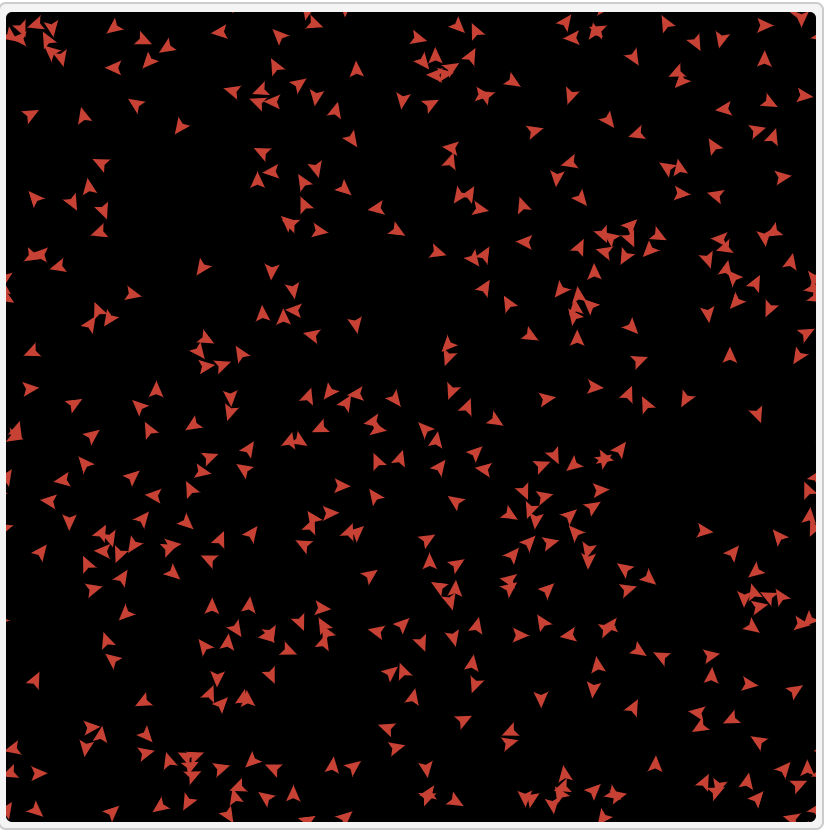
\includegraphics[width=0.4\textwidth]{figures/net0.png}} 
    \subfigure[]{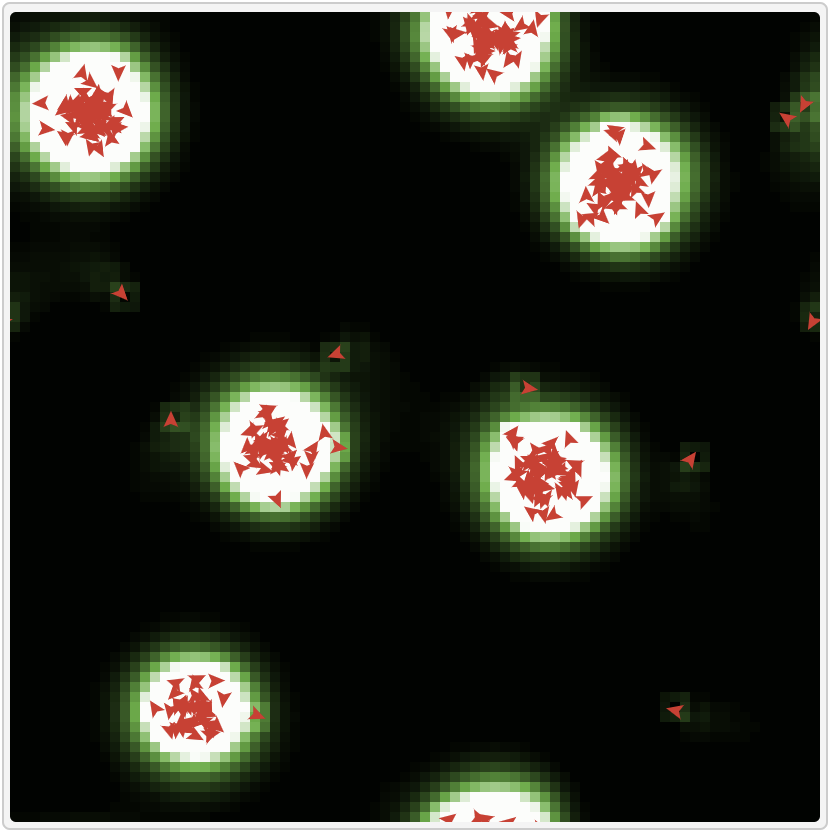
\includegraphics[width=0.4\textwidth]{figures/netF.png}} 
    \caption{Simulazione di riferimento}\label{fig:refsimfoto}
\end{figure}
La simulazione\footnote{\url{https://www.netlogoweb.org/launch\#http://www.netlogoweb.org/assets/modelslib/Sample\%20Models/Biology/Slime.nlogo}}
utilizzata come riferimento per questo progetto di tesi è presente nella libreria
di modelli di NetLogo. Il modello di riferimento è ``Slime''\space\cite{wilensky1997netlogo}\space\cref{fig:refsimfoto}.
e per simulare l'aggregazione di tanti singoli organismi in un gruppo vengono usati gli agenti sopra descritti, 
ovvero le \textit{patch} e le \textit{tartarughe}.
Quest'ultime si muovono in uno spazio a griglia e durante il loro movimento rilasciano una particolare molecola
chiamata ``feromone'' che si deposita in una posizione precisa. L'intero mondo è quindi suddiviso
in tantissime ``micro-aree'' chiamate \textit{patch}\space\cref{fig:patch}. La \textit{tartaruga} per muoversi 
``annusa'' davanti a se, ovvero percepisce se nelle \textit{patch} vicine è presente del ``feromone''. Se il valore di quest'ultimo è abbastanza alto, la 
\textit{tartaruga} si sposterà nella posizione ``annusata'', mentre, in caso contrario la \textit{tartaruga} si muoverà in modo randomico nello spazio circostante. 
Durante tutto ciò, le \textit{patches} diffonderanno del ``feromone'' alle varie posizioni vicine e, con il passare del tempo,
il ``feromone'' tende ad evaporare (ovvero sparire) dalla griglia.

\begin{figure}[ht]
    \centering
    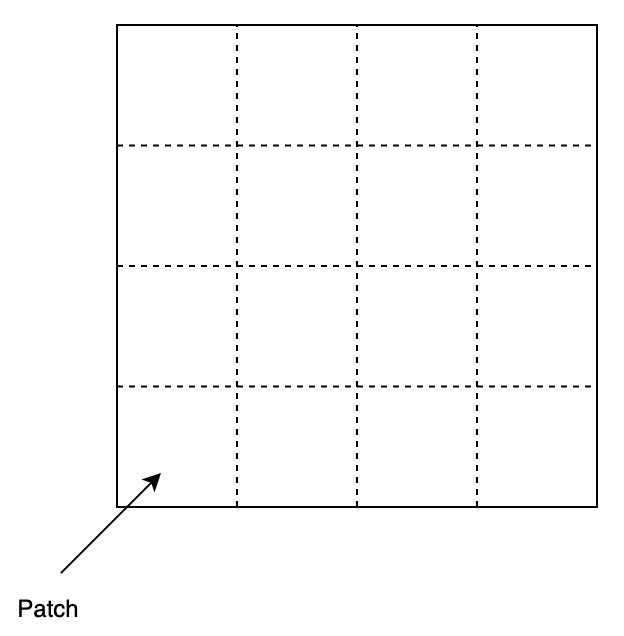
\includegraphics[scale=0.6]{figures/patch.png}
    \caption{Il mondo suddiviso in patch}\label{fig:patch}
\end{figure}

\section{Overview su \textit{slime-mold}}
Nel contesto della presente tesi, sulla base della simulazione di riferimento\ref{refSim} e i comportamenti osservati in essa, si è scelto di indagare un altro 
fenomeno dalle caratteristiche estremamente simili: la muffa mucillaginosa.
In natura, l'aggregazione delle cellule di muffa mucillaginosa (detti anche funghi mucillaginosi o, in inglese, \textit{slime-mold}) rappresenta
comportamento in cui entità individuali interagiscono tra di loro per formare strutture complesse e funzionali. 
Lo \textit{slime-mold} è un organismo unicellulare ma, talvolta, può trovarsi anche ad agire come un'entità multicellulare. 
Pur non essendo un fungo è spesso classificato nella stessa categoria per via delle sue caratteristiche affini a quelle di questi organismi.
La particolarità principale della muffa mucillaginosa è che può comportarsi come un organismo unicellulare o multicellulare a seconda delle diverse 
condizioni ambientali in cui si trova.
L'habitat principale di questi organismi è il terreno umido, dove di solito si nutrono di foglie morte o di tronchi di alberi in putrefazione.
Quando trova una fonte di cibo, lo \textit{slime-mold} si aggrega, formando una massa citoplasmatica detta ``plasmodio'', composta da un grande numero cellule. Inoltre,
questa massa può muoversi, ``navigando'' attraverso il terreno in cerca di cibo.
Infatti, se le risorse alimentari scarseggiano o l'ambiente diventa meno ospitale, lo \textit{slime-mold} può assumere forme diverse: può formare spore, 
resistenti per sopravvivere in condizioni avverse, oppure aggregarsi insieme ad altri individui simili per formare una struttura multicellulare
che si comporta come un'unica entità, condividendone di conseguenza risorse e compiti.

\section{Alchemist}
Alchemist\space\cite{Pianini_2013} è un simulatore DES (Discrete Event System) che estende il modello computazionale 
base delle reazioni chimiche in modo tale da favorirne l'applicabilità a situazioni complesse,
pur mantenendo elevate prestazioni. In particolare, Alchemist si fonda su una versione ottimizzata 
dell'algoritmo di Gillespie\cite{gillespie1977exact} chiamata Next Reaction Method\cite{gibson2000efficient}, esteso in modo tale da poter lavorare 
con un ambiente agile e dinamico dove è possibile aggiungere o rimuovere reazioni, dati e
connessioni topologiche. Le applicazioni già implementate sono varie e comprendono, ad esempio, 
simulazioni di reazioni biochimiche e movimento di pedoni. Il punto di forza del sistema è il 
meta-modello estremamente astratto, la cui effettiva realizzazione è demandata alle ``incarnazioni'',
le quali rappresentano l'implementazione vera e propria delle diverse categorie di simulazioni 
eseguibili all'interno. Attualmente troviamo 4 incarnazioni: 
\begin{itemize}
    \item Protelis
    \item SAPERE
    \item Biochemistry
    \item Scafi
\end{itemize}
\subsection{Il meta-modello} 
Come accennato in precedenza, il meta-modello \cref{fig:alchemist} è uno dei punti di forza maggiori di Alchemist. 
Per meta-modello si intende un tipo di paradigma che descrive la struttura, le regole e le relazioni
che i modelli di dati devono seguire all'interno di un sistema. Rappresenta in modo astratto i 
concetti e le relazioni all'interno del dominio di interesse e stabilisce i vincoli e le convenzioni
che tutti i modelli devono usare. Dunque, tutte le incarnazioni sviluppate presentano le stesse entità
``base''. Poichè Alchemist è sviluppato partendo da un'ispirazione orientata alla chimica/biochimica,
le entità presentano nomi riconducibili a quei mondi. Infatti troviamo:
\begin{itemize}
    \item \textbf{Molecole} (\textit{molecule}): il nome di un dato, concettualmente interpretabile come il nome di una variabile.
    \item \textbf{Concentrazioni} (\textit{concentration}): il valore associato alla molecola.
    \item \textbf{Nodi}\label{node} (\textit{node}): il ``contenitore'' di molecole e reazioni.
    \item \textbf{Ambiente} (\textit{environment}): l'astrazione dello spazio; è un “contenitore” di nodi e svolge i seguenti compiti:
    \begin{itemize}
        \item Restituire la posizione dei nodi.
        \item Restituire la distanza tra due nodi.
        \item Supportare il movimento dei nodi, se presente.
    \end{itemize}
    \item \textbf{Vicinato} (\textit{neighborhood}): un entità composta da un nodo centrale e un insieme di nodi vicini.
    \item \textbf{Regola di collegamento} (\textit{linking rule}): una funzione relativa allo stato corrente dell'ambiente che associa ad ogni nodo un vicinato.
    \item \textbf{Reazione} (\textit{reaction}): un qualsiasi evento che provoca un cambiamento dello stato dell'ambiente \cref{fig:alchemist}. È definita da una lista di condizioni, una o più lista di azioni e una distribuzione temporale. La frequenza con la quale avviene una reazione dipende da:
    \begin{itemize}
        \item Un parametro statico ``rate''.
        \item Il valore di ogni condizione.
        \item Una ``rate equation'', ovvero una equazione che combina il parametro statico (rate) con i valori delle condizioni, restituendo un ``instantaneous rate''.
        \item Una distribuzione temporale.
    \end{itemize}
    \item \textbf{Condizione} (\textit{condition}): una funzione che, dato lo stato attuale del'ambiente (environment), restituisce un booleano ed un numero. Se il booleano è falso la reazione non può avvenire. In caso contrario, invece, avviene. Il numero può invece influenzare la velocità della reazione a seconda della reazione e della distribuzione temporale.
    \item \textbf{Azione} (\textit{action}): un cambiamento nell'ambiente.
\end{itemize}
\begin{figure}[ht]
    \centering
    \subfigure[]{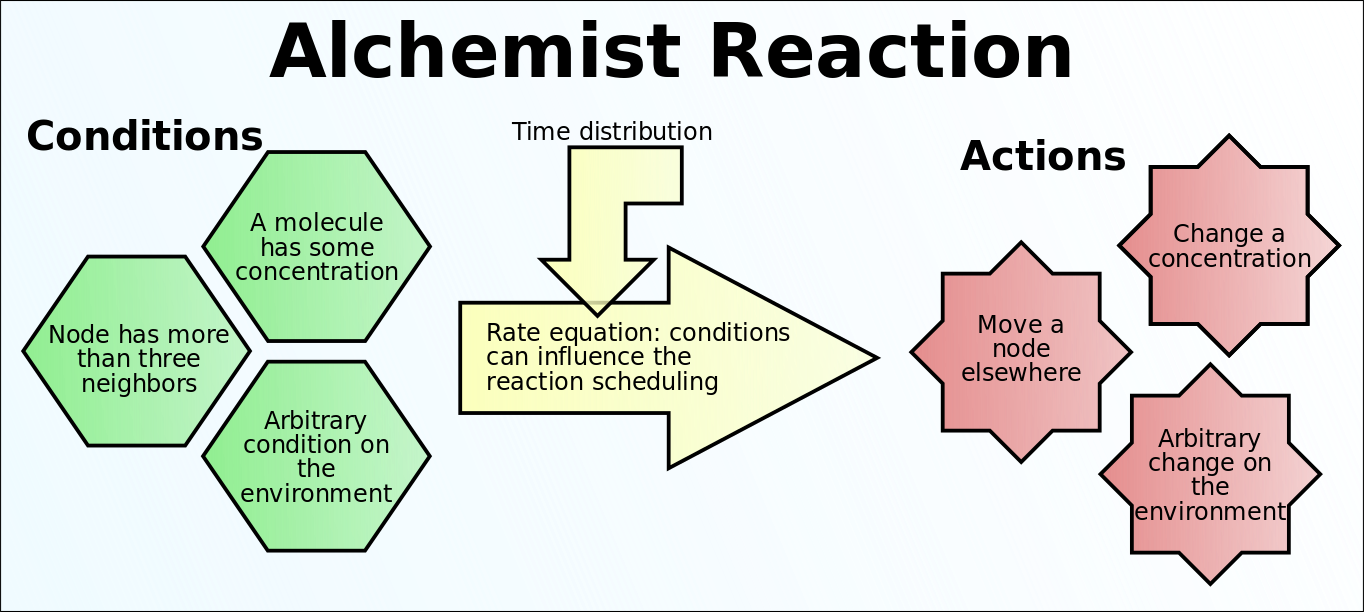
\includegraphics[width=0.49\textwidth]{figures/alchemistReaction.png}} 
    \subfigure[]{\includegraphics[width=0.49\textwidth]{figures/alchemistModel.png}} 
    \caption{(a) Reazione in Alchemist (b) Il modello di alchemist}\label{fig:alchemist}
\end{figure}
\clearpage





\chapter{Analisi del dominio}
\section{Dominio}
Il dominio di interesse è caratterizzato dalla presenza di entità, vive e in movimento, in un ambiente.
Durante il loro movimento rilasciano una traccia,
sotto forma di sostanza chimica,
simile ad un odore che può essere percepito dalle altre entità presenti nell'area circostante. Questa sostanza
si deposita in un punto dell'ambiente ed inizia ad espandersi. Con il passare del tempo la sostanza, evaporando, svanisce dall'ambiente.
Quando un'entità, muovendosi, percepisce la presenza di questa sostanza, viene spinta a muoversi verso la direzione 
in cui l'ha percepita. Questo comportamento, riprodotto in larga scala, porta alla formazione di strutture complesse e funzionali.
Un esempio di questo comportamento è osservabile in natura, nel caso delle formiche: queste, infatti, riescono a 
creare disposizioni complesse e funzionali per tracciare il cibo e per costruire i loro nidi.
\section{Requisiti}
Analizzando il dominio possiamo individuare e sintetizzare
le caratteristiche e i requisiti che la simualzione dovrà avere:
\begin{itemize}
    \item Entità ``vive'', che si muovono e depositano il feromone.
    \item Un ambiente che gestisce la presenza del feromone; in particolare questo deve:
    \begin{itemize}
        \item Permettere il depositarsi della sostanza.
        \item Diffondere la sostanza.
        \item Far evaporare la sostanza.
    \end{itemize}
    \item Le entità devono avere un concetto di direzione.
    \item Il movimento deve seguire delle regole ben precise.
\end{itemize}

Segue uno schema generale del dominio, rappresentato in figura\space\ref{fig:generale}.
\begin{figure}[ht]
    \centering
    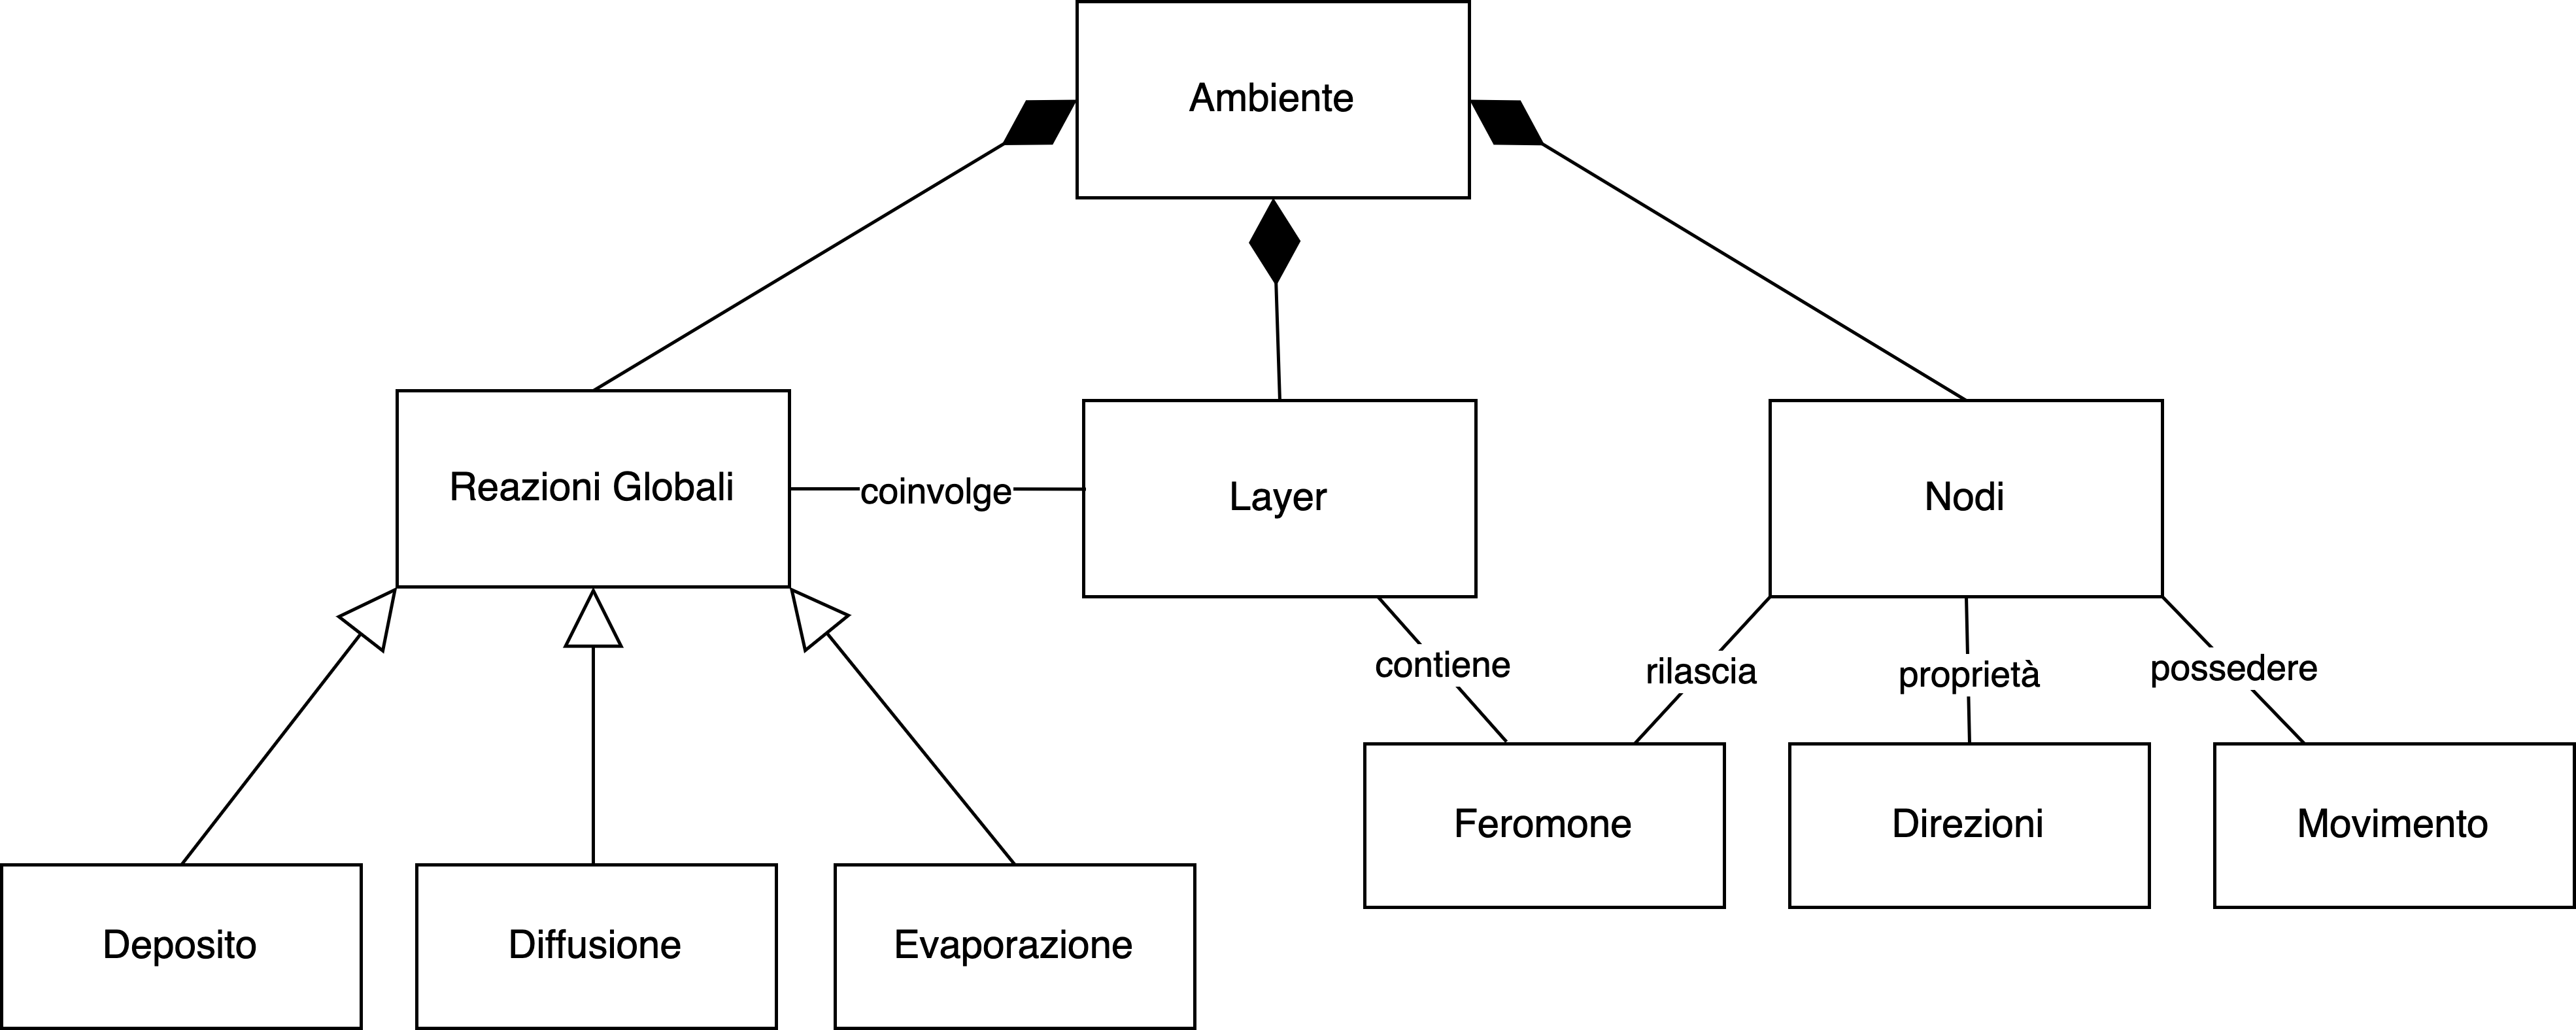
\includegraphics[width=0.9\textwidth]{figures/generale.png}
    \caption{Schema geneale del dominio.}\label{fig:generale}
\end{figure}\newline

Non sono stati individuati ulteriori requisiti specifici per la realizzazione di questo progetto di tesi.
Lo scopo di questa ricerca, infatti, è stato soprattutto quello di comprendere come il simulatore Alchemist 
potesse essere in grado di simulare questi comportamenti, tramite lo sviluppo un modello
dimostrativo.
\chapter{Design}
\section{Layer}
Si pensi alla simulazione come se fosse un micro-mondo, una ``città'' complessa
e ricca di informazioni. È di interesse capire il livello di temperatura oppure di inquinamento nelle varie aree cittadine, dati invisibili
all'occhio umano ma comunque presenti nell'ambiente e percepibili da chi lo abita. Si ha bisogno
di inserire nell'ambiente degli ``strati'' invisibili che hanno il compito di raccogliere queste informazioni.
È possibile, in Alchemist, definire questi ``strati'' di dati, chiamati Layer.
\newline
Nel contesto di questo progetto è stato necessario l'utilizzo di un Layer che avesse la funzione di ``rete di raccolta''
dei feromoni che, nella simulazione di riferimento\space\ref{refSim}, venivano rilasciati dalle \textit{tartarughe} nelle varie posizioni
dello spazio. In questo caso il layer ha la stessa dimensione dell'ambiente, in modo tale da poter suddividere l'intera area nelle varie \textit{patch} di cui si 
è discusso sopra.
Il layer, chiamato \textit{PheromoneLayer} ha come compiti:
\begin{itemize}
    \item Implementare una struttura dati per tenere traccia della quantità di feromone presente in ogni posizione.
    \item Offrire un modo per aggiornare i valori del feromone.
    \item Condividere con le altre classi la struttura dati contenente la quantità di feromone per una specifica posizione.
    \item Lasciare la possibilità all'utente di decidere le dimensioni dell'area totale di riferimento e di ogni \textit{patch}.
\end{itemize}
Di seguito si riporta un diagramma UML \cref{fig:phLayer} che rappresenta il layer.
\begin{figure}[ht]
    \centering
    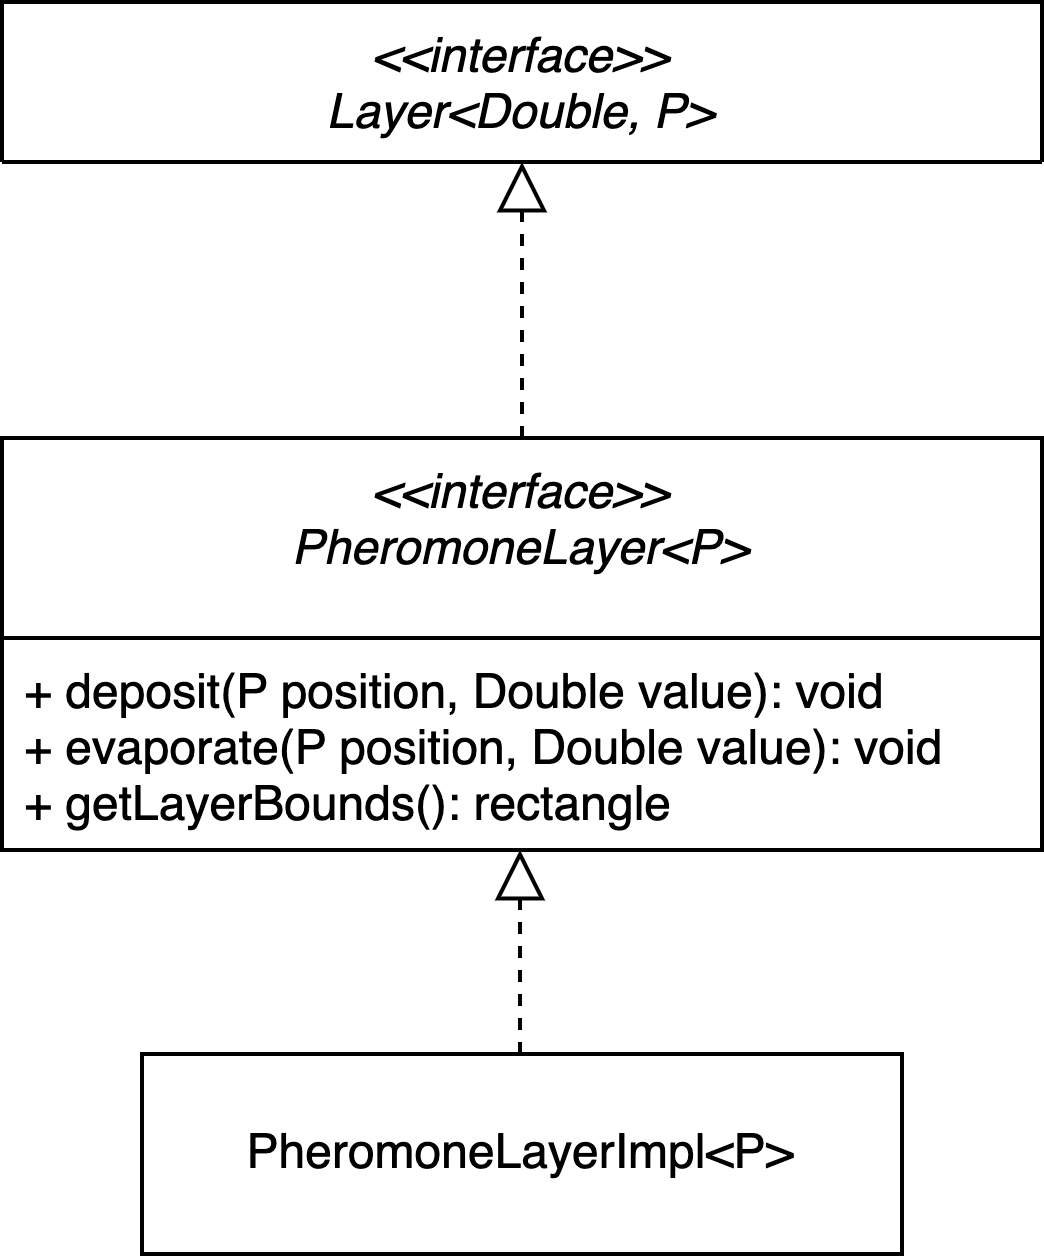
\includegraphics[width=.5\linewidth]{figures/pheromoneLayer.png}
    \caption{Struttura PheromoneLayer}\label{fig:phLayer}
\end{figure}

\subsection{Le posizioni}
Un aspetto di particolare rilevanza è stato il processo decisionale relativo alla gestione delle posizioni collegate 
al deposito del feromone. Nella simulazione di riferimento\space\ref{refSim} si trova uno spazio a griglia, dove l'area totale è suddivisa
in ``micro-aree'' chiamate \textit{patch}. In Alchemist, tuttavia, non è presente il concetto di ``area'' o ``spazio'', necessario per individuare una \textit{patch},
in quanto le posizioni sono puntiformi e non necessariamente hanno coordinate intere. Il layer sviluppato ricalca l'area (rettangolare o quadrata) del sistema iniziale,
implementando anche un sistema di conversione che trasforma la posizione puntiforme in modo tale da emulare la presenza di una ``area'' bidimensionale, a forma di quadrato, che corrisponde alla \textit{patch}.
Entrambe le misure, ovvero quella della griglia e quella della \textit{patch} sono dinamiche e possono essere modificate dall'utente.
\section{I nodi}
Una volta definito l'ambiente di simulazione è importante determinare la struttura e la logica delle 
entità che lo abiteranno. Nella simulazione di riferimento\space\ref{refSim} è possibile individuare come abitanti le \textit{tartarughe}
che, muovendosi, rilasciano una traccia chimica chiamata ``feromone''. Dunque, concettualmente, la \textit{tartaruga} è un ``contenitore'' infinito di 
feromoni e, muovendosi, ne rilascia una parte nell'ambiente. Alchemist possiede il concetto di nodo\space\ref{node} che, per definizione, 
è un contenitore di molecole che vive in un ambiente. È stato quindi necessario solamente definire la tipologia di molecola
appartenente al nodo per tradurre questo aspetto della simulazione (ma anche del mondo reale) in Alchemist.

\begin{figure}[ht]
    \centering
    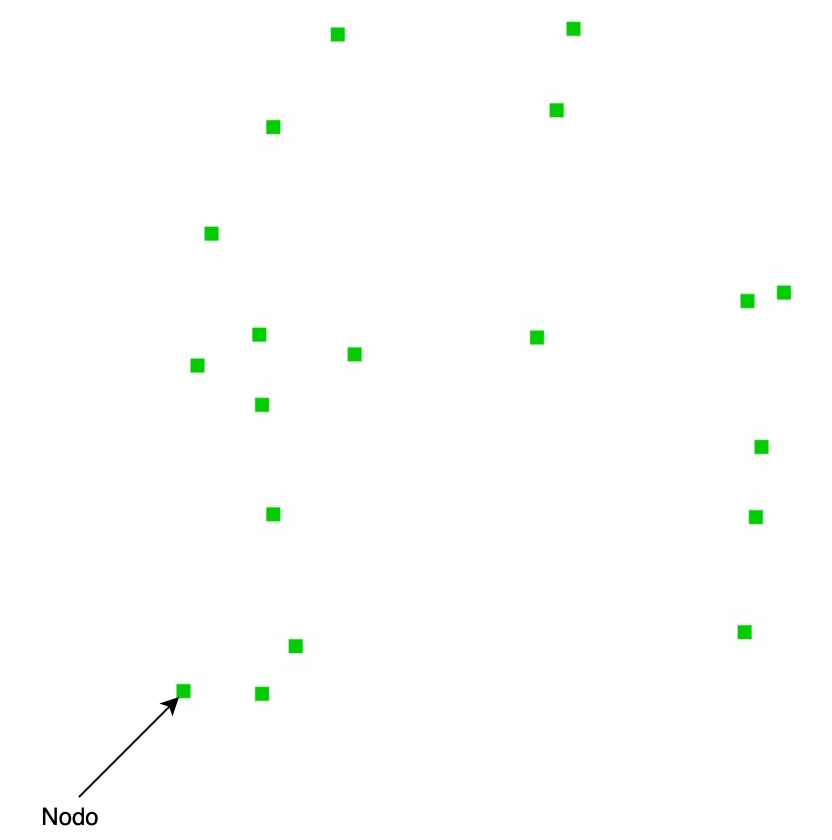
\includegraphics[width=.5\linewidth]{figures/nodes.png}
    \caption{Rappresentazione grafica dove ogni punto è un nodo.}\label{fig:nodes}
\end{figure}

\section{Direzioni}
Un aspetto importante da considerare è la direzione del movimento delle \textit{tartarughe}. Nella simulazione di riferimento\space\ref{refSim} le \textit{tartarughe}
si muovono e seguono un percorso che deriva dalla loro direzione. Essendo questo un attributo proprio delle \textit{tartarughe},
è stato necessario sviluppare una soluzione che permettesse di inizializzare i nodi della simulazione con delle direzioni facilmente accessibili 
e modificabili in base alle esigenze.

Alchemist rende possibile la definizione di attributi personalizzati per i nodi, chiamati \textit{Node Property}. Il corretto utilizzo di questa
funzionalità ha permesso di definire un attributo di tipo \textit{Direction} per ogni nodo che rappresentasse la direzione 
in modo tale da poter simulare in modo realistico questo aspetto della simulazione.

%\section{Il movimento}

\section{Reazioni globali}
La Reazione Globale o \textit{Global Reaction} rappresenta uno strumento fondamentale per descrivere
le interazioni e i processi che avvengono all'interno di un sistema simulato.
Possono essere utilizzate per modellare una vasta gamma di fenomeni, dalla diffusione chimica alla dinamica dei sistemi biologici.
Contrariamente alle reazioni locali, le \textit{Global Reaction} hanno effetti concreti sull'intero contesto in esame. 
Realizzare una modellazione precisa e realistica di questi fenomeni può essere di grande interesse per indagare tutti i risultati possibili.
\begin{figure}[ht]
    \centering
    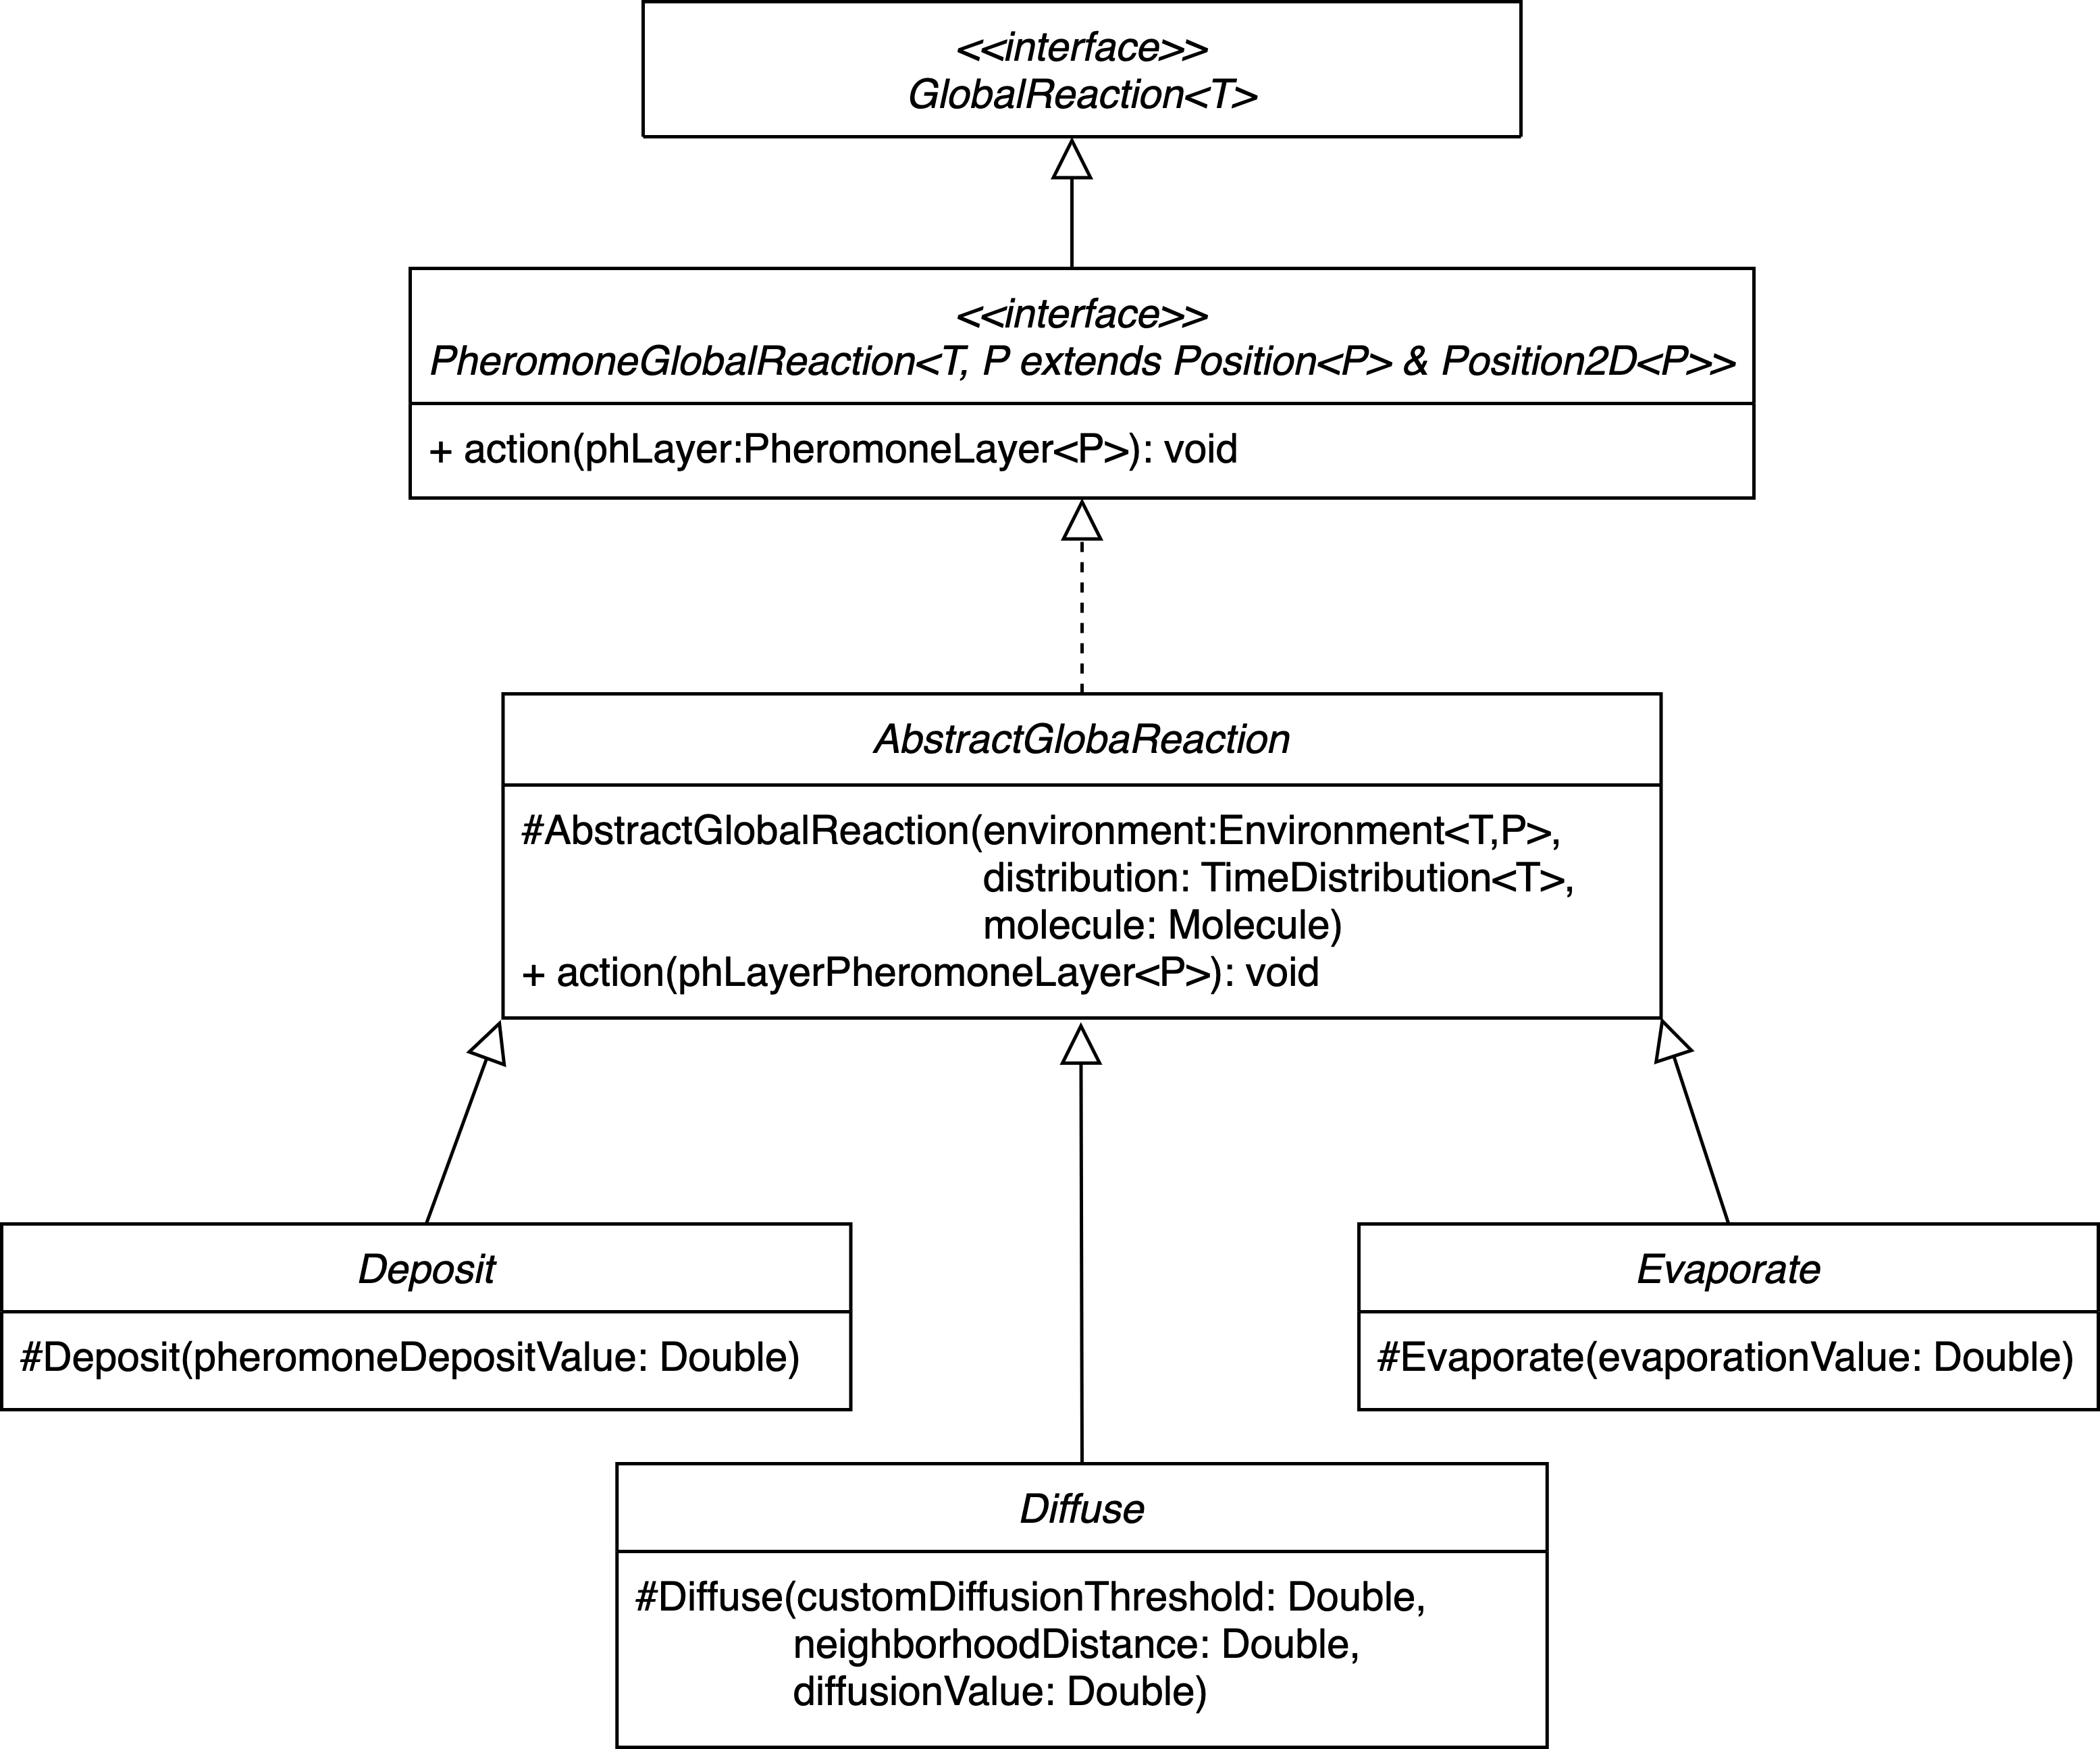
\includegraphics[width=.7\linewidth]{figures/global.png}
    \caption{Schema delle Global Reaction }\label{fig:global}
\end{figure}\newline
Come si vede in figura \cref{fig:global}, nell'ambito di questa tesi si individuano 3 tipi di reazioni, tutte collegate ai feromoni:
\begin{itemize}
    \item Rilascio (\textit{Deposit})
    \item Evaporazione (\textit{Evaporation})
    \item Diffusione (\textit{Diffusion})
\end{itemize}

\subsection{Rilascio}
Questa reazione coinvolge in modo diretto il nodo, l'ambiente e il layer. Durante ogni movimento il nodo rilascia 
nell'ambiente una certa quantità di feromone in una posizione discreta. Il layer si occupa della raccolta del feromone,
posizionandolo in una \textit{patch} ed incrementando il valore della sostanza collegato ad essa.
\subsection{Evaporazione}
L'evaporazione riguarda solamente il layer. In natura, con il passare del tempo, la traccia chimica diventa sempre più
lieve fino a sparire completamente. Questa reazione si occupa esattamente di questo: ogni \textit{patch} caratterizzata
dalla presenza di un livello di feromone positivo viene individuata e il valore collegato ad essa viene decrementato in modo graduale.
\subsection{Diffusione}
La diffusione \cref{fig:diffusion} del feromone è un evento che caratterizza in modo diretto il layer e i nodi. Ogni volta che il nodo rilascia il feromone e
questo si deposita in una \textit{patch}, il layer diffonde nelle \textit{patches} vicine delle tracce dello stesso.
\begin{figure}[ht]
    \centering
    \subfigure[]{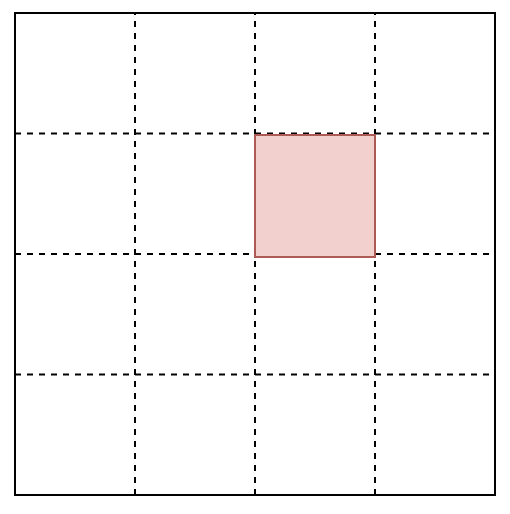
\includegraphics[width=0.3\textwidth]{figures/dif0.png}} 
    \subfigure[]{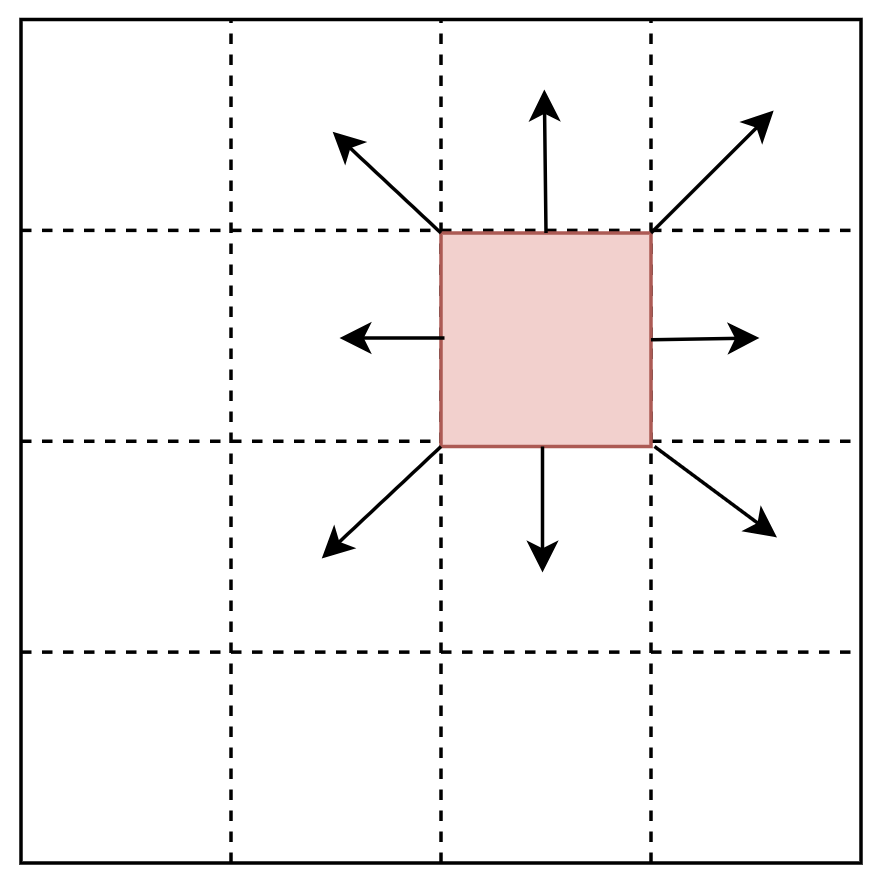
\includegraphics[width=0.3\textwidth]{figures/diffusione.png}} 
    \subfigure[]{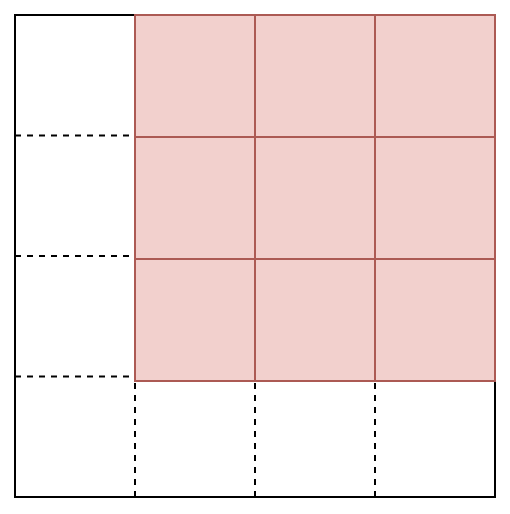
\includegraphics[width=0.3\textwidth]{figures/difF.png}} 
    \caption{Il processo di diffusione; la figura (a) mostra il feromone in una \textit{patch}, la figura (b) mostra le \textit{patch} vicine nelle 
    quali il feromone verrà diffuso e la figura (c) mostra lo stato dell'ambiente una volta che la diffusione è terminata.}\label{fig:diffusion}
\end{figure}

\chapter{Implementazione}
\section{Struttura del progetto}
La struttura del progetto, organizzato in package, è la seguente:
\begin{itemize}
    \item \textbf{Layer}: il layer personalizzato della simulazione.
    \item \textbf{Actions}: le azioni della simulazione.
    \item \textbf{GlobalReactions}: le azioni globali della simulazione.
    \item \textbf{NodeProperty}: le proprietà dei nodi della simulazione.
\end{itemize}
Per avviare il progetto in Alchemist, è necessario delineare accuratamente i parametri
e le opzioni desiderate attraverso un file di configurazione YAML\@. Questo file fornisce
le istruzioni necessarie per definire il comportamento del simulatore, specificare
i componenti del sistema e regolare le interazioni tra di essi.

\section{Layer}\label{layer}
Il \texttt{PheromoneLayer<P extends Position2D<P>>}, layer personalizzato della simulazione, è stato implementato 
come un'interfaccia che estende \texttt{Layer<T, P>} - interfaccia propria di Alchemist - 
dove \texttt{T} è il tipo di nodo e \texttt{P} è il tipo di posizione. 
L'utilizzo del parametro \texttt{P} implica che il \texttt{PheromoneLayer} può essere utilizzato con qualsiasi tipo di posizione, ma, nel contesto di questa tesi,
si è preferito sfruttare posizioni \texttt{Position2D<P>} bidimensionali.
Per la sua creazione è necessario definire 5 misure:
\begin{itemize}
    \item \texttt{startX}: la coordinata x di partenza.
    \item \texttt{startY}: la coordinata y di partenza.
    \item \texttt{width}: la larghezza del layer.
    \item \texttt{height}: l'altezza del layer.
    \item \texttt{step}: la dimensione del passo, ovvero la lunghezza del lato di ogni \textit{patch}.
\end{itemize}
Lo \texttt{step} è un parametro fondamentale per la corretta implementazione della simulazione
in quanto Alchemist non possiede il concetto di area, necessaria per individuare una \textit{patch}.
Queste vengono rappresentate come ``aree'' puntiformi, e la loro dimensione (ovvero la distanza di un punto dall'altro) è appunto definita da questo parametro.
Nella simulazione, il nodo deposita il feromone in una qualsiasi posizione, discreta e non obbligatoriamente intera, all'interno dei limiti dello spazio, e il \texttt{PheromoneLayer} 
si occupa di convertire questa posizione in una appartenente ad una \textit{patch}. 
Il \texttt{PheromoneLayer} esegue, quindi, un arrotondamento per eccesso o per difetto, in modo tale da ottenere la posizione della \textit{patch} più vicina.
\begin{figure}[ht]
    \centering
    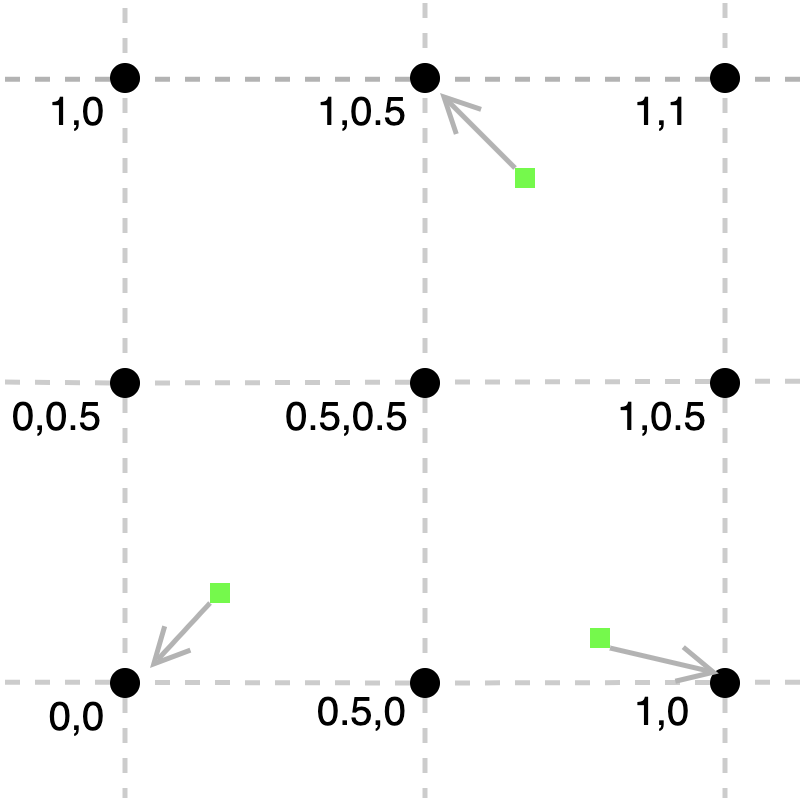
\includegraphics[width=.3\linewidth]{figures/patch-nodi.png}
    \caption{Rappresentazione grafica delle \textit{patches} puntiformi. Ogni punto rappresenta una patch,
    mentre i quadratini rappresentano i nodi e la freccia indica su che \textit{patch} il nodo depositerà il feromone. In questo esempio
    startX e startY hanno come valore 0, width e height 1 e step 0.5}\label{fig:patch-nodi}
\end{figure}
%devo parlare della Mappa e delle posizioni, di come vengono convertite magari aggiungendo delle foto.

\subsection{Struttura dati}\label{strDati}
Un aspetto di fondamentale importanza riguarda la struttura dati utilizzata per la gestione del feromone.
Per ovviare alla mancanza del concetto di area, è stato utilizzato un \texttt{HashMap<P, Double>} che associa ad ogni posizione \texttt{P} un valore \texttt{Double} di feromone.
Questa mappa viene inizializzata nel costruttore della classe attraverso il metodo \texttt{setupEnviromnent()} che si occupa di popolare la mappa
con tutte le possibili posizioni delle \textit{patch} e di inizializzare il feromone a 0.\newline

\lstinputlisting[language=Java,label={lst:phlayer}]{listings/phlayerSetup.java}

\subsection{Metodi}
I metodi definiti nell'interfaccia e implementati nella classe sono:
\begin{itemize}
    \item \texttt{void evaporate(P position, Double value)}: metodo che permette di far evaporare il feromone. 
    Richiede in input la posizione e il valore del feromone.
    \item \texttt{void deposit(P position, Double value)}: metodo che permette di depositare il feromone.
     Richiede in input la posizione e il valore del feromone.
    \item \texttt{Rectangle getLayerBounds()}: metodo che restituisce un oggetto di tipo \texttt{Rectangle}, contentente i parametri per delineare l'area del Layer.
\end{itemize}
Di grande importanza sono i primi due metodi: \texttt{evaporate} e \texttt{deposit}.
Entrambi sono nominati come le reazioni globali della simulazione e vengono utilizzati dalle stesse per accedere la mappa e modificare il feromone.\newline
\lstinputlisting[language=Java,label={lst:phlayer}]{listings/phLayerDepositAndEvaporate.java}

\section{Actions}
In questa sezione vengono descritte le azioni della simulazione. Possiamo trovare:
\begin{itemize}
    \item \texttt{MoveNode}: azione che permette ad ogni singolo nodo di muoversi.
    \item \texttt{NodeInfo}: azione che permette di controllare le informazioni di ogni singolo nodo.
\end{itemize}

\subsection{MoveNode}\label{moveNode}
La classe \texttt{MoveNode<P extends Position<P> \& Position2D<P>>} incorpora l'intera logica che permette il movimento di ogni singolo nodo. 
Per la sua creazione è necessario che l'utente definisca i seguenti parametri:
\begin{itemize}
    \item \texttt{sniffThreshold}: la soglia di feromone che il nodo deve percepire per potersi muovere.
    \item \texttt{sniffDistance}: la distanza del passo di movimento.
    \item \texttt{wiggleBias}: la tendenza a preferire un movimento casuale oscillatorio in una direzione specifica.
\end{itemize}
Il parametro \texttt{wiggleBias} può essere impostato in 3 modi:
\begin{itemize}
    \item \texttt{0}: il nodo ha il 50\% di muoversi in avanti e il 25\% di muoversi a destra o a sinistra.
    \item \texttt{0 > x <= 40}: il nodo tende a preferire la direzione di sinistra; il valore indica la probabilità di muoversi in quel verso.
    Il valore 40 indica il 100\% di probabilità di muoversi in quella direzione.
    \item \texttt{-40 => x < 0}: il nodo tende a preferire la direzione di destra; il valore indica la probabilità di muoversi in quel verso.
    Il valore -40 indica il 100\% di probabilità di muoversi in quella direzione.
\end{itemize}
La classe \texttt{MoveNode} estende la classe astratta \texttt{AbstractAction<T>}, facente parte del set base di Alchemist, implementandone i metodi astratti.
Tra questi, il metodo \texttt{execute} è il più importante, in quanto si occupa di eseguire l'azione di movimento vera e propria.
La logica di movimento segue questi passi:
\begin{enumerate}
    \item Viene individuata la posizione attuale del nodo.
    \item Questa posizione viene adattata alla \textit{patch} più vicina.
    \item Vengono calcolate le direzioni possibili in base alle patch adiacenti alla posizione calcolata precedentemente che hanno una 
    concentrazione di feromone superiore ad una soglia definita dall'utente (il parametro si chiama \texttt{sniffThreshold}).
    \item Viene identificata la \textit{patch} con la maggiore concentrazione di feromone. Tuttavia, questa, non è sempre individuabile. Vi sono due casi possibili: nel primo, 
        nella \textit{patch} è presente un valore di feromone, ma esso è sotto la soglia minima \texttt{sniffThreshold} e dunque la \textit{patch} viene scartata;
         nel secondo caso, invece, nella \textit{patch} non è presente alcuna traccia di feromone, e dunque questa non viene proprio rilevata.
    \item Se la \textit{patch} è presente:
    \begin{enumerate}
        \item La direzione del nodo viene aggiornata in base alla direzione della \textit{patch} con la maggiore concentrazione di feromone.
        \item Il nodo si muove verso quella \textit{patch} e si aggiorna la direzione del nodo.
    \end{enumerate}
    \item Se la \textit{patch} non è presente:
    \begin{enumerate}
        \item Viene calcolata una direzione casuale tra quelle possibili (dritto, verso destra o verso sinistra a seconda del valore del parametro \texttt{wiggleBias}),
        tenendo in considerazione la direzione attuale del nodo.
        \item Il nodo si muove nella direzione scelta e l'orientamento del nodo viene aggiornato.
    \end{enumerate}
\end{enumerate}

\subsection{NodeInfo}
La classe \texttt{NodeInfo<T, P extends Position<P> \& Position2D<P>>} permette di tracciare le informazioni di ogni singolo nodo, come
raffigurato in figura\space\cref{fig:nodeinfo}. Anche questa
classe estende la classe astratta \texttt{AbstractAction<T>}, implementandone i metodi. Le informazioni osservabili sono le seguenti:
\begin{itemize}
    \item \texttt{PheromoneValue}: la concentrazione di feromone nella \textit{patch} in cui si trova il nodo.
    \item \texttt{direction}: la direzione attuale del nodo.
    \item \texttt{pheromone}: la quantità di feromone che il nodo rilascia.
\end{itemize}
\begin{figure}
    \centering
    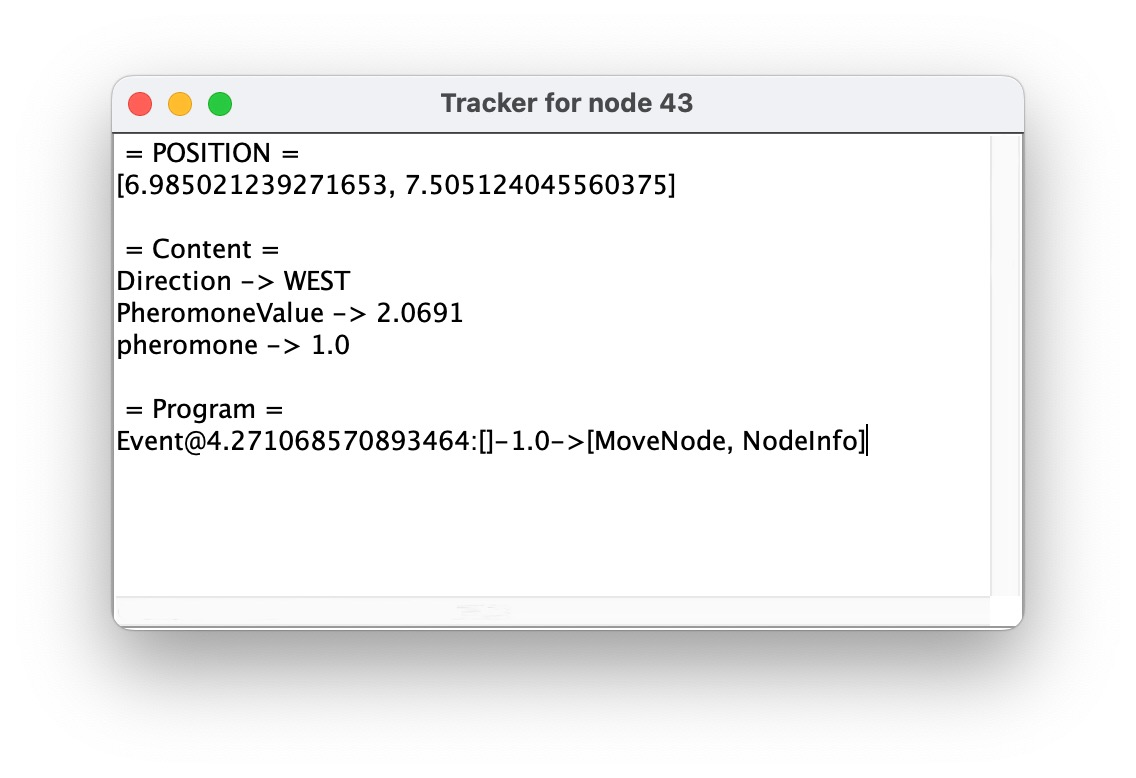
\includegraphics[width=.7\linewidth]{figures/nodeinfo.jpg}
    \caption{Le informazioni del nodo. Si possono osservare nella sezione ``Content''}\label{fig:nodeinfo}
\end{figure}
\clearpage

\section{GlobalReactions}
In questa sezione del progetto sono state implementate le reazioni globali della simulazione. Possiamo trovare:
\begin{itemize}
    \item \texttt{Evaporate}: azione che permette di far evaporare il feromone.
    \item \texttt{Deposit}: azione che permette di far diffondere il feromone.
    \item \texttt{Diffuse}: azione che diffonde il feromone nelle \textit{patch} adiacenti.
\end{itemize}
Le classi sopra introdotte estendono la classe astratta \texttt{AbstractGlobalReaction<T, P extends Position<P>}
\& \texttt{Position2D<P>}
la quale implementa l'interfaccia \newline\texttt{PheromoneGlobalReaction<T, P>}. Quest'ultima estende l'interfaccia 
propria di Alchemist \texttt{GlobalReaction<T>} dove sono definite le operazioni da implementare in modo tale che il 
simulatore possa identificare ed utilizzare in modo corretto tutti i sorgenti necessari.
L'interfaccia \texttt{PheromoneGlobalReaction<T, P>} definisce il metodo \texttt{action(PheromoneLayerImpl<P> phLayer)}.
Quest'ultimo è implementato in ogni classe e si occupa di eseguire la logica della reazione.
Si è scelta questa struttura in quanto i metodi definiti dall'interfaccia \texttt{GlobalReaction<T>}
sono i medesimi per ogni azione globale e quindi l'utilizzo della classe astratta \texttt{AbstractGlobalReaction},
che li implementa, permette di evitare la ripetizione inutile del codice.

La simulazione esegue una volta al secondo le reazioni in modo tale da garantire un'evoluzione corretta del feromone nel tempo. Inoltre, le reazioni
in questione vengono eseguite nell'ordine in cui sono state definite nel file di configurazione YAML\@.
\subsection{Evaporate}
Questa classe ha il compito di fare evaporare il feromone dall'ambiente. L'azione di evaporazione è simulata
attraverso la moltiplicazione del valore del feromone per un coefficente di evaporazione compreso tra 0 e 1, 
definito dall'utente. Questo evento ha effetto su ogni singola \textit{patch} in cui è presente il feromone.
Per alterare il valore del feromone di ogni \textit{patch}, viene richiamato il metodo 
\texttt{evaporate} del \texttt{PheromoneLayer}\space\ref{layer}.
\newline
\lstinputlisting[language=Java,label={lst:evaporate}]{listings/evaporate.java}[ht]

\subsection{Deposit}
Il sorgente protagonista di questa sotto-sezione compie l'azione di depositare il feromone. Dall'ambiente
vengono individuate le posizioni di tutti i nodi e viene poi richiamato il metodo \texttt{deposit} del \texttt{PheromoneLayer}\space\ref{layer}
per modificare il valore del feromone, associato alla posizione attuale del nodo, presente nella struttura dati\space\ref{strDati}.\newline
\lstinputlisting[language=Java,label={lst:deposit}]{listings/deposit.java}

\subsection{Diffuse}
Quest'ultima classe si occupa di diffondere il feromone nelle \textit{patch} adiacenti. Vengono quindi individuate tutte
le \textit{patch}, e per ognuna si calcola il suo vicinato. Se la \textit{patch} ha un valore di feromone superiore ad una soglia definita dall'utente,
si procede a diffondere il feromone. La diffusione è emulata attraverso la moltiplicazione del valore del feromone
per un coefficente di diffusione deciso dall'utente. Questa reazione, concettualmente, è simile alla \texttt{Deposit} in quanto
nel vicinato di una \textit{patch} viene depositato del feromone, e per questo motivo, viene richiamato il metodo \texttt{deposit} del \texttt{PheromoneLayer}\space\ref{layer}.
\newline
\lstinputlisting[language=Java,label={lst:diffuse}]{listings/diffuse.java}

\section{NodeProperty}
La classe \texttt{DirectionProperty} è stata implementata per poter associare ad ogni nodo una proprietà che rispecchiasse la sua direzione attuale.
Estende la classe \texttt{AbstractNodeProperty<T>} fornita dal set base di Alchemist.
L'enum \texttt{Direction}, che definisce le direzioni possibili in cui un nodo può muoversi, è propedeutico all'utilizzo di questa classe.
L'enum definisce i 4 punti cardinali e i loro punti intermedi. Infatti, un nodo può muoversi in 8 direzioni diverse e, tenere traccia di
queste, è fondamentale per la corretta esecuzione della simulazione. L'enum, oltre a contenere le definizioni delle direzioni, contiene anche,
per ognuna di esse, metodi che ne ritornano le coordinate x e y e le direzioni adiacenti. All'avvio del programma, ad ogni nodo 
viene assegnata una direzione in modo randomico. 

La \texttt{NodeProperty} è una proprietà fondamentale per il corretto funzionamento dell'azione \texttt{MoveNode}
\space\ref{moveNode}; senza di essa, infatti, il movimento del nodo risulterebbe irrealistico in quanto si muoverebbe in modo completamente casuale.
Con l'implementazione di questa classe e una logica di movimento (implementata nella classe \texttt{MoveNode}\space\ref{moveNode})
pensata per sfruttare questa componente, invece,
si osserva che il movimento di un singolo nodo risulta piuttosto ``armonioso'' e realistico, più simile a quello di un essere vivente che 
esplora l'ambiente circostante.


\chapter{Valutazioni}
In questa sezione vengono presentati i risultati delle simulazioni effettuate e i loro valori.
Nella \cref{risultati} ad ogni simulazione è associata una serie di immagini che mette in luce i risultati ottenuti.
\section{Simulazione 1}\label{sim1}
I valori di questa simulazione\space \cref{fig:sim1} sono i seguenti:
\begin{table}[ht]
    \centering
    \caption{Valori dei parametri}
    \begin{tabular}{ll}
        \toprule
        Parametro                   & Valore \\
        \midrule
        Numero di nodi              & 500    \\
        \texttt{sniffThreshold}     & 1.5    \\
        \texttt{wiggleBias}         & 0      \\
        \texttt{evaporation}        & 0.6    \\
        \texttt{diffusion}          & 0.5    \\
        \texttt{deposit}            & 1      \\
        \texttt{startX}             & -15    \\
        \texttt{startY}             & -15    \\
        \texttt{width}              & 30     \\
        \texttt{height}             & 30     \\
        \texttt{step}               & 0.5    \\
        \texttt{customDiffusionTreshold} & 5 \\
        \bottomrule
    \end{tabular}\label{tab:parametri1}
\end{table}\newline
Dalle dimensioni dell'ambiente si può osservare che il numero di \textit{patches} è pari a 3721. A tutti questi punti è assegnato il compito di 
immagazzinare la quantità di feromone depositata dai nodi. 
Data l'alta densità di punti di raccolta del feromone ci si aspetta che l'aggregazione avvenga abbastanza rapidamente e in zone ben definite. 
L'alto numero di nodi, 500 nell'esempio, promette una situazione in cui i nodi vicini tra loro rimangano ``intrappolati'' nelle loro posizioni, continuando a depositare il feromone e 
generando un piccolo ``nucleo'' di aggregazione. Una volta formato tale agglomerato, tutti i nodi che si trovano nelle vicinanze ne saranno attratti
e contriburanno a rafforzare l'aggregazione.


\section{Simulazione 2}\label{sim2}
I valori di questa simulazione\space \cref{fig:sim2} sono i seguenti:
\begin{table}[ht]
    \centering
    \caption{Valori dei parametri}
    \begin{tabular}{ll}
        \hline
        Parametro                   & Valore \\
        \hline
        Numero di nodi              & 500    \\
        \texttt{sniffThreshold}     & 4      \\
        \texttt{wiggleBias}         & 0      \\
        \texttt{evaporation}        & 0.6    \\
        \texttt{diffusion}          & 0.0625 \\
        \texttt{deposit}            & 1      \\
        \texttt{startX}             & -15    \\
        \texttt{startY}             & -15    \\
        \texttt{width}              & 30     \\
        \texttt{height}             & 30     \\
        \texttt{step}               & 0.5    \\
        \texttt{customDiffusionTreshold} & 1 \\
        \hline
    \end{tabular}\label{tab:parametr2}
\end{table}\newline
Questa simulazione presenta valori molti simili a quelli della precedente, ma con un valore di \texttt{sniffThreshold} più alto e un valore di \texttt{diffusion} più basso.
Il risultato atteso vede un processo di aggregazione più lento dove i nodi si muovono per più tempo nello spazio prima di aggregarsi o di trovare un 
agglomerato già presente e che, generalmente, ci saranno meno zone di aggregazione. Quelle che si formano 
tenderanno a contenere un grande numero di nodi: sarà necessario che questi si incontrino in un unico punto per formare un cluster.

\section{Simulazione 3}\label{sim3}
I valori di questa simulazione\space \cref{fig:sim3} sono i seguenti:
\begin{table}[ht]
    \centering
    \caption{Valori dei parametri}
    \begin{tabular}{ll}
        \toprule
        Parametro                   & Valore \\
        \midrule
        Numero di nodi              & 100    \\
        \texttt{sniffThreshold}     & 1.5    \\
        \texttt{wiggleBias}         & 0      \\
        \texttt{evaporation}        & 0.6    \\
        \texttt{diffusion}          & 0.5    \\
        \texttt{deposit}            & 1      \\
        \texttt{startX}             & -15    \\
        \texttt{startY}             & -15    \\
        \texttt{width}              & 30     \\
        \texttt{height}             & 30     \\
        \texttt{step}               & 0.5    \\
        \texttt{customDiffusionTreshold} & 5 \\
        \bottomrule
    \end{tabular}\label{tab:parametri3}
\end{table}\newline
Questa simulazione dimostra che, pur con un numero di nodi estremamente inferiore rispetto ai precedenti esempi,
l'aggregazione avviene in ogni caso.
Si osserva che, dopo 100 secondi, si iniziano a formare piccole aggregazioni in pochissimi punti dello spazio.
Dopo 300 secondi si può notare che l'aggregazione si è rafforzata in quei punti, ma sono presenti ancora diversi nodi in movimento.


\section{Simulazione 4}\label{sim4}
Questa simulazione presenta gli stessi valori della seconda simulazione\space(\cref{sim2}), ma con un numero di nodi pari a 100.
Lo scopo di questa simulazione è quello di confrontare i risultati con la terza simulazione\space(\cref{sim3}), che presenta gli stessi valori della prima simulazione\space(\cref{sim1}),
ma con differenze nel \texttt{sniffThreshold} e \texttt{diffusion}. In questo caso non avviene alcuna aggregazione e 
il motivo principale è legato alle differenze di valori di \texttt{sniffThreshold} e \texttt{diffusion}.

I valori di questa simulazione\space \cref{fig:sim4} sono i seguenti:
\begin{table}[ht]
    \centering
    \caption{Valori dei parametri}
    \begin{tabular}{ll}
        \hline
        Parametro                   & Valore \\
        \hline
        Numero di nodi              & 100    \\
        \texttt{sniffThreshold}     & 4      \\
        \texttt{wiggleBias}         & 0      \\
        \texttt{evaporation}        & 0.6    \\
        \texttt{diffusion}          & 0.0625 \\
        \texttt{deposit}            & 1      \\
        \texttt{startX}             & -15    \\
        \texttt{startY}             & -15    \\
        \texttt{width}              & 30     \\
        \texttt{height}             & 30     \\
        \texttt{step}               & 0.5    \\
        \texttt{customDiffusionTreshold} & 1 \\
        \hline
    \end{tabular}\label{tab:parametri4}
\end{table}

\section{Simulazione 5}\label{sim5}
I valori di questa simulazione\space \cref{fig:sim5} sono i seguenti:
\begin{table}[ht]
    \centering
    \caption{Valori dei parametri}
    \begin{tabular}{ll}
        \hline
        Parametro                   & Valore \\
        \hline
        Numero di nodi              & 500    \\
        \texttt{sniffThreshold}     & 4      \\
        \texttt{wiggleBias}         & 0      \\
        \texttt{evaporation}        & 0.5    \\
        \texttt{diffusion}          & 1 \\
        \texttt{deposit}            & 2      \\
        \texttt{startX}             & -10    \\
        \texttt{startY}             & -10    \\
        \texttt{width}              & 20     \\
        \texttt{height}             & 20     \\
        \texttt{step}               & 0.5    \\
        \texttt{customDiffusionTreshold} & 10 \\
        \hline
    \end{tabular}\label{tab:parametri5}
\end{table}\newline
Quest'ultima simulazione presenta valori diversi da quelle precedenti. Si è voluto indagare il caso
in cui si avesse un ambiente più piccolo e dei valori di \texttt{evaporation}, \texttt{diffusion} e \texttt{deposit} 
più alti. Con questa configurazione si osserva una quasi immediata aggregazione dei nodi in tanti punti: questo comportamento
era atteso dati i valori di partenza.


\section{Risultati delle simulazioni}\label{risultati}
\begin{figure}[ht]
    \centering
    \subfigure[]{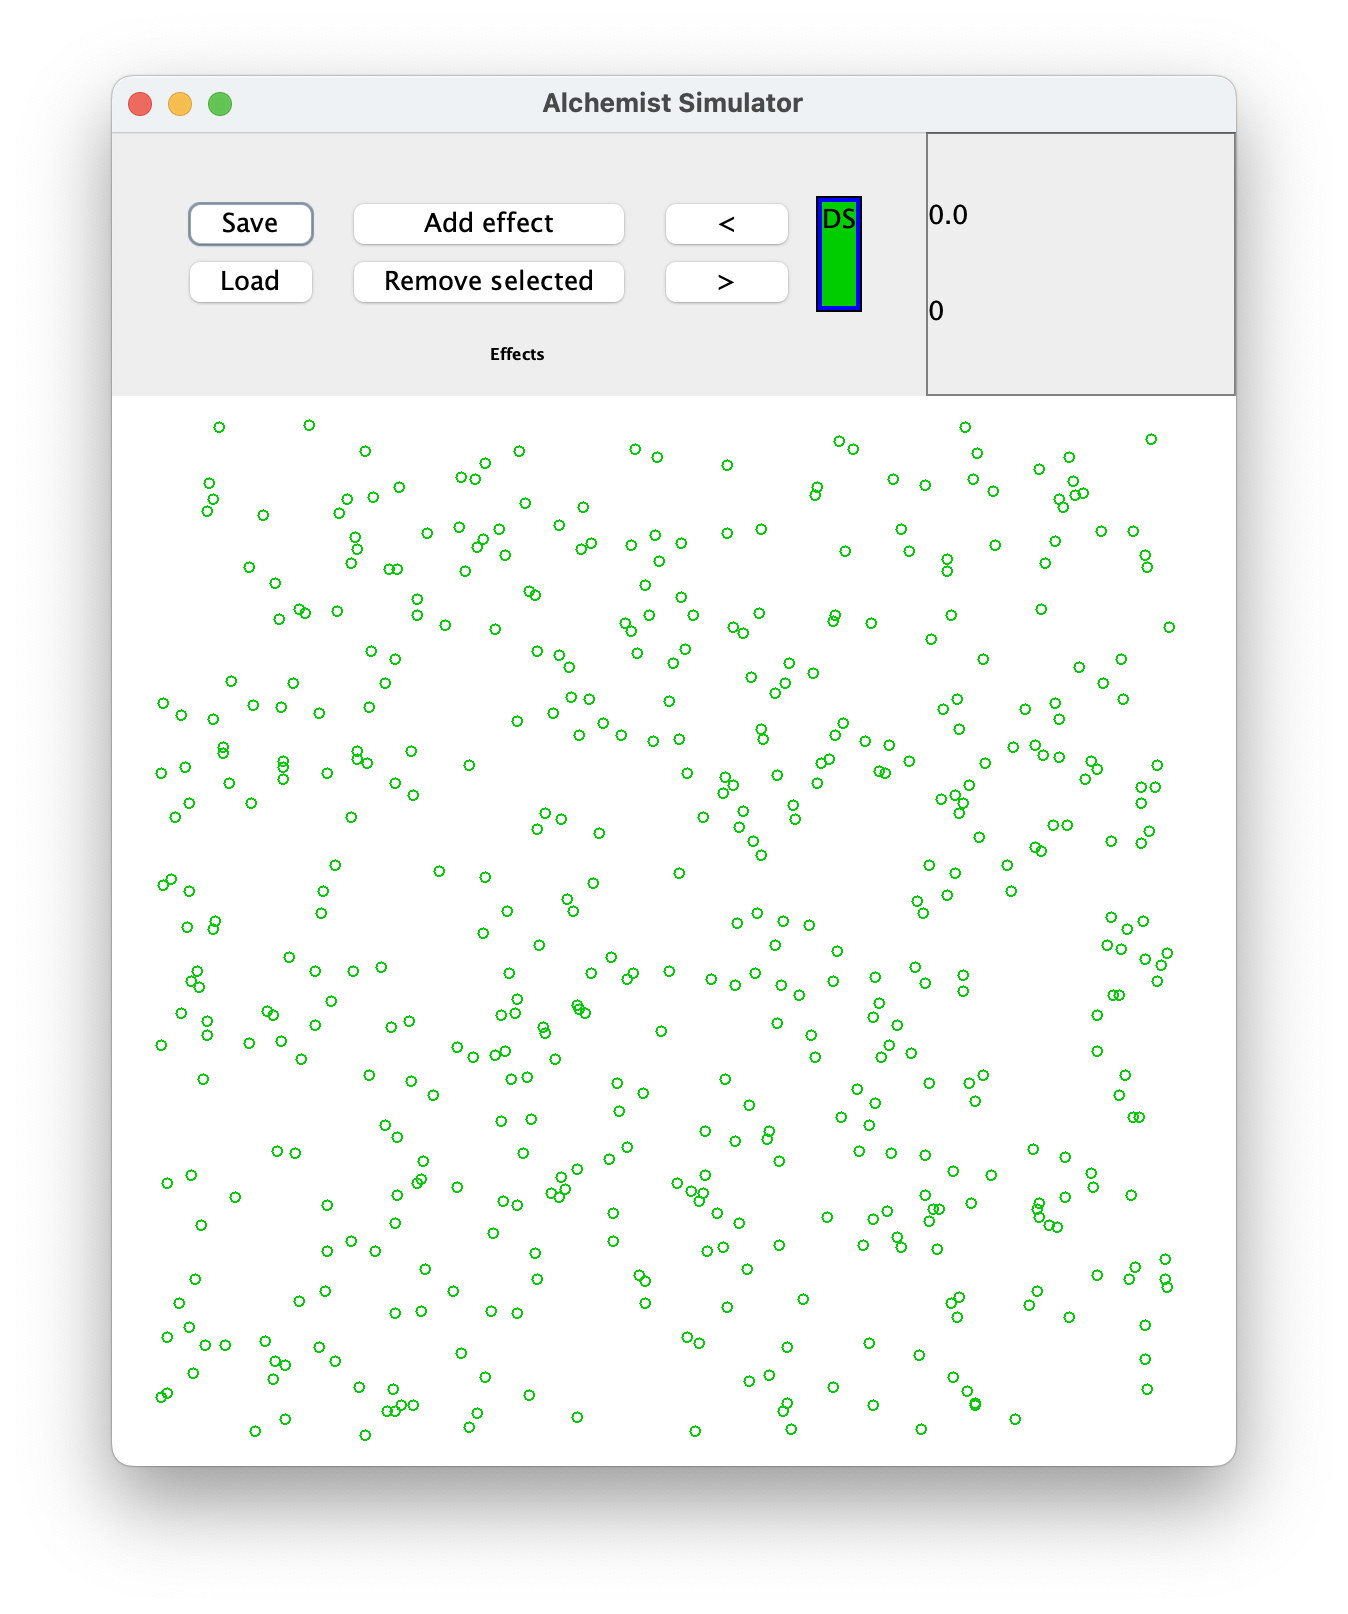
\includegraphics[width=0.32\textwidth]{figures/rect0.png}} 
    \subfigure[]{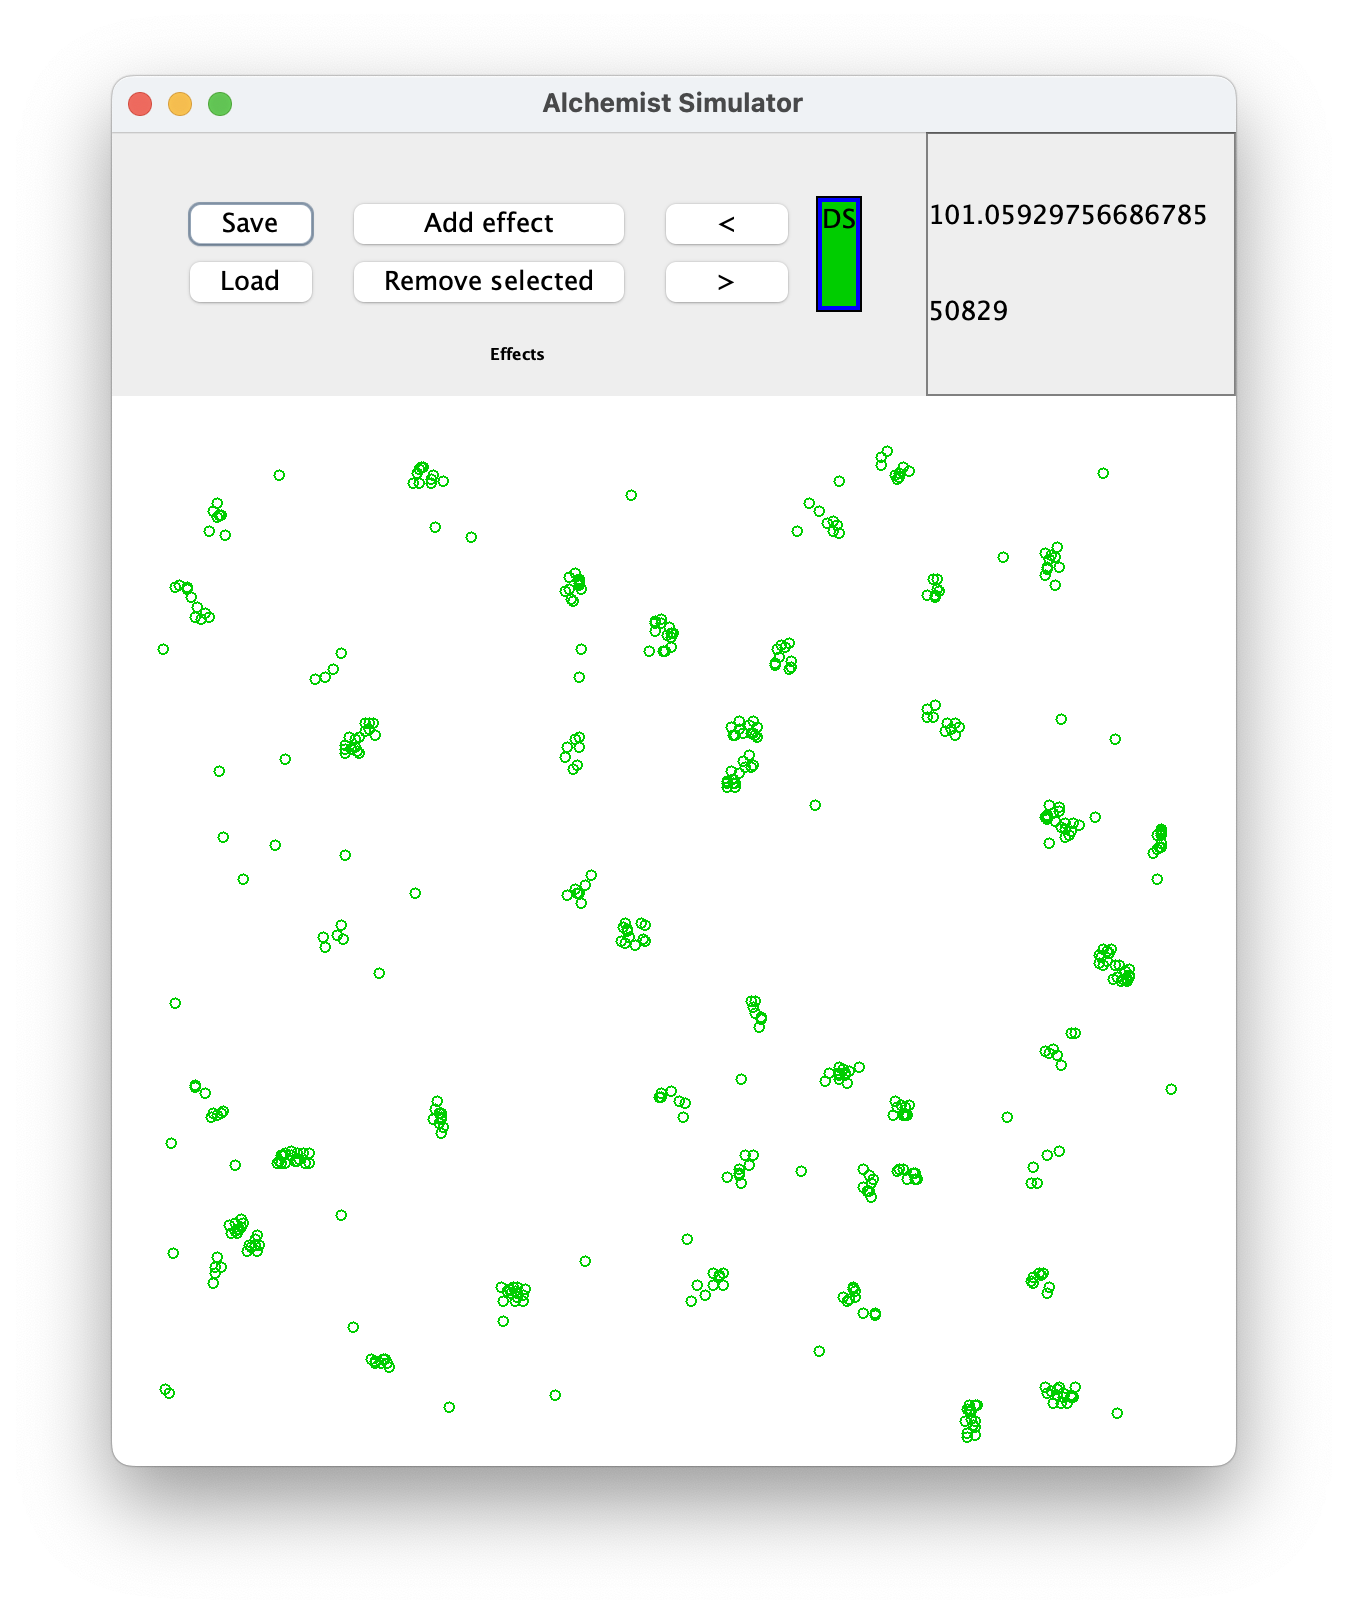
\includegraphics[width=0.32\textwidth]{figures/rect100.png}} 
    \subfigure[]{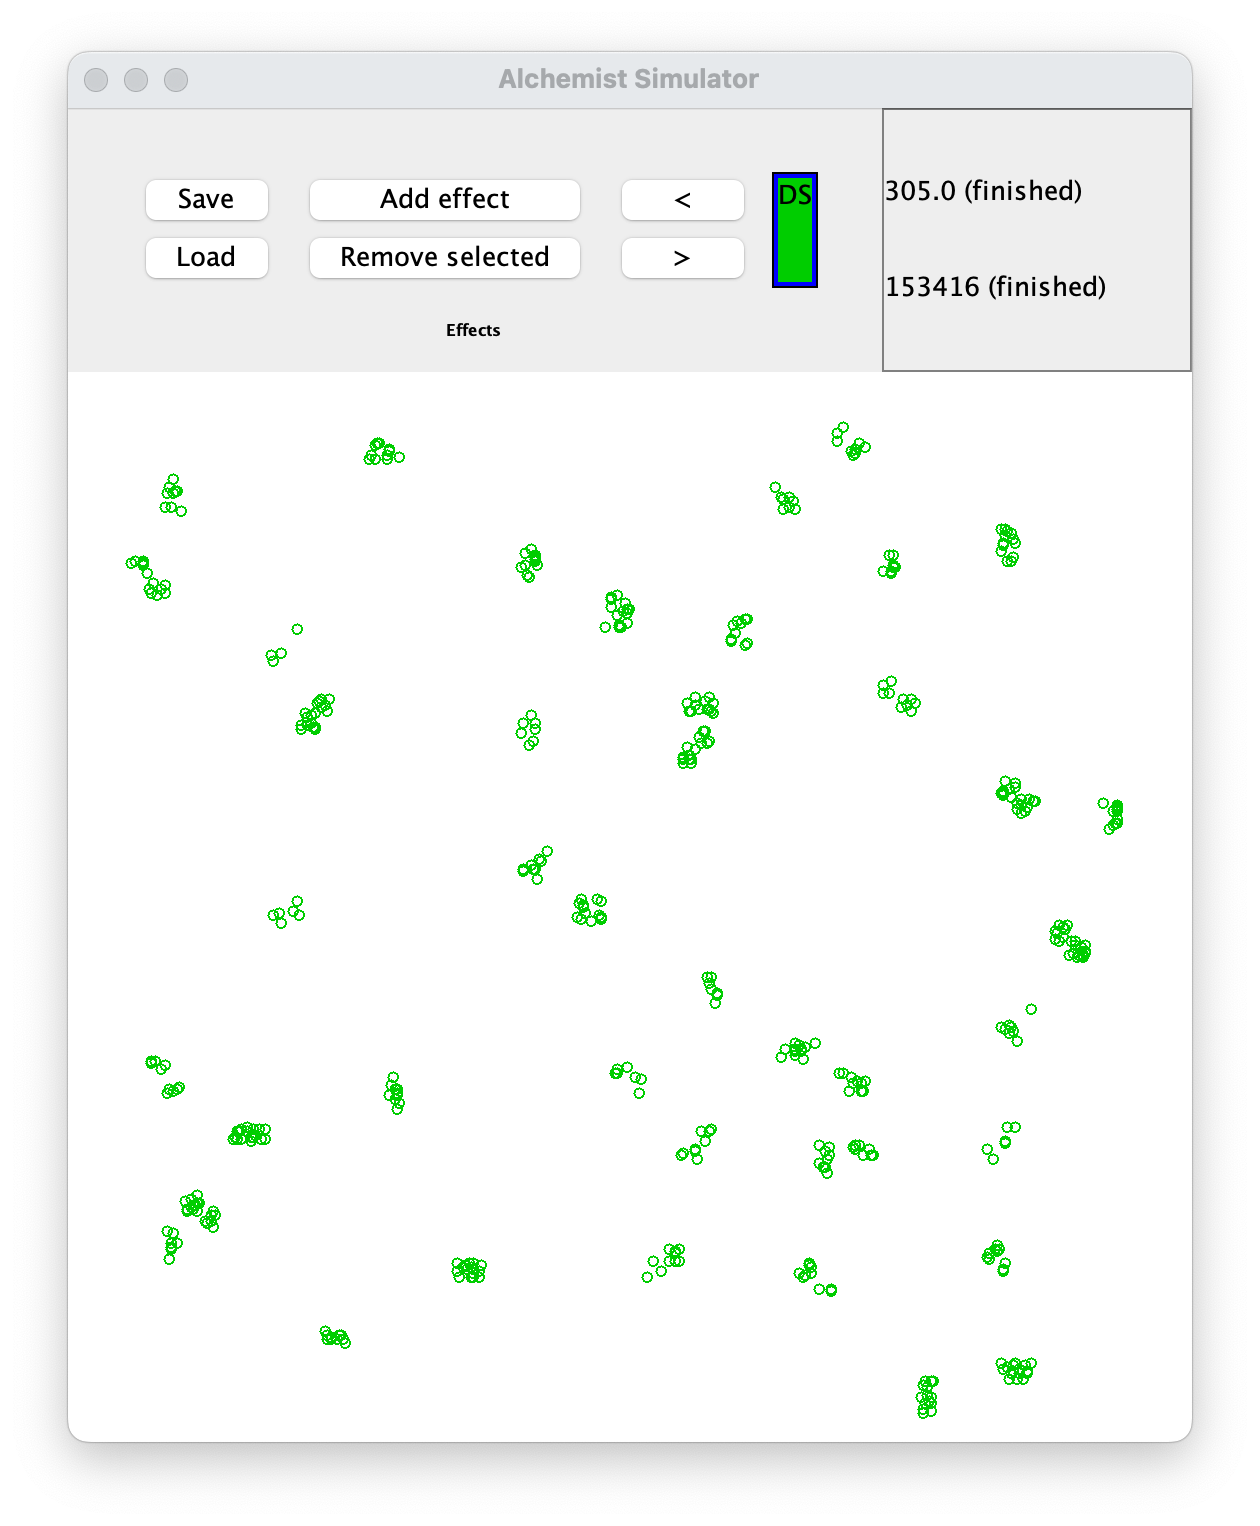
\includegraphics[width=0.32\textwidth]{figures/rectFine.png}}
    \caption{(a) Inizio (b) Dopo 100 secondi (c) Dopo 300 secondi}\label{fig:sim1}
\end{figure}
\begin{figure}[ht]
    \centering
    \subfigure[]{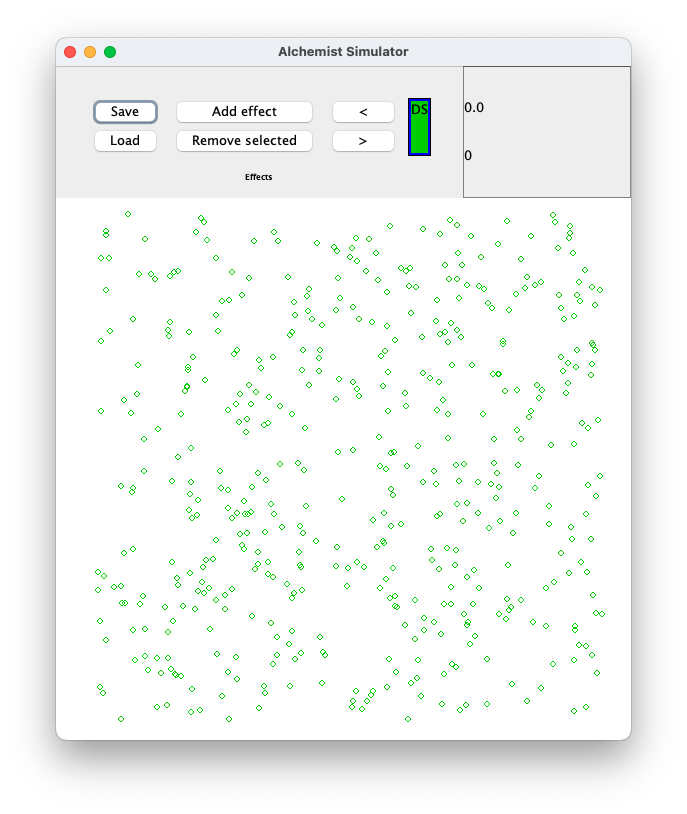
\includegraphics[width=0.32\textwidth]{figures/slow0.png}} 
    \subfigure[]{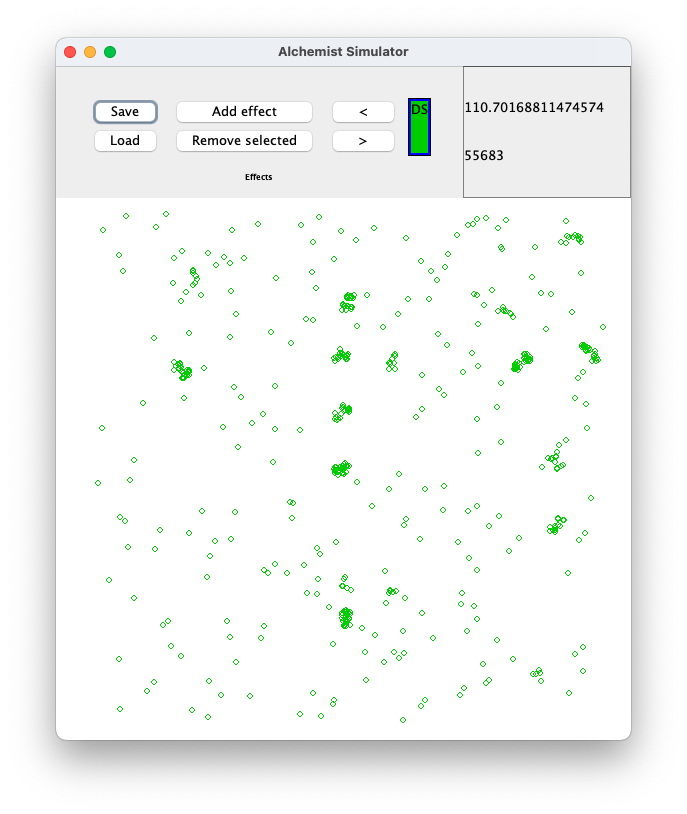
\includegraphics[width=0.32\textwidth]{figures/slow100.png}} 
    \subfigure[]{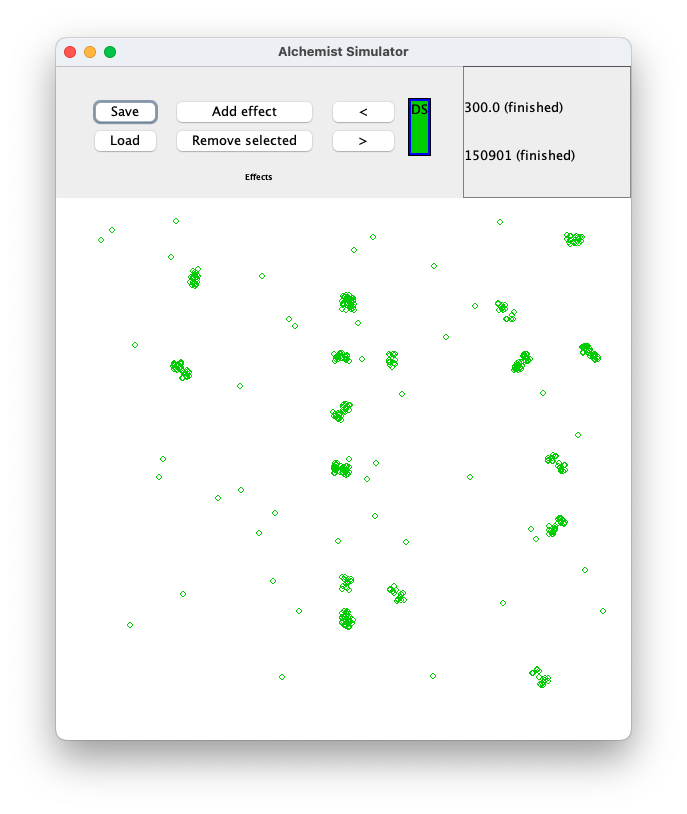
\includegraphics[width=0.32\textwidth]{figures/slowF.png}}
    \caption{(a) Inizio (b) Dopo 100 secondi (c) Dopo 300 secondi}\label{fig:sim2}
\end{figure}
\begin{figure}[ht]
    \centering
    \subfigure[]{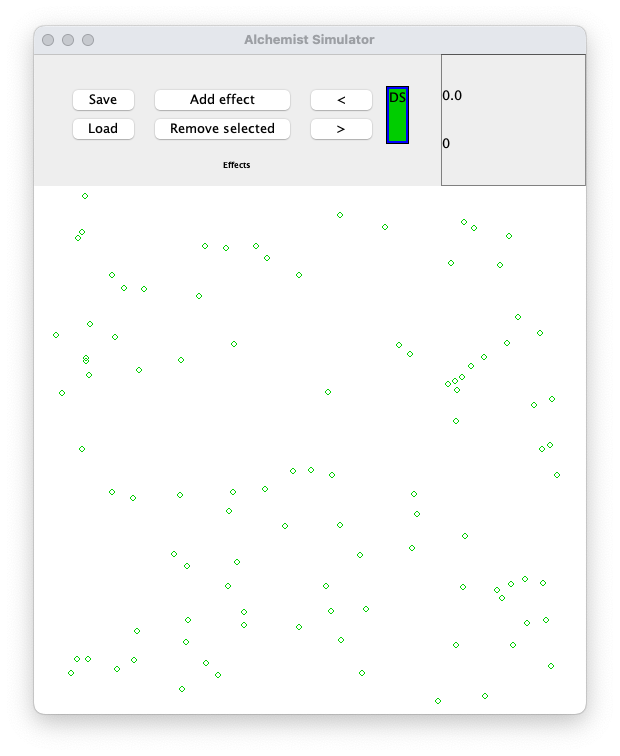
\includegraphics[width=0.32\textwidth]{figures/cento0.png}} 
    \subfigure[]{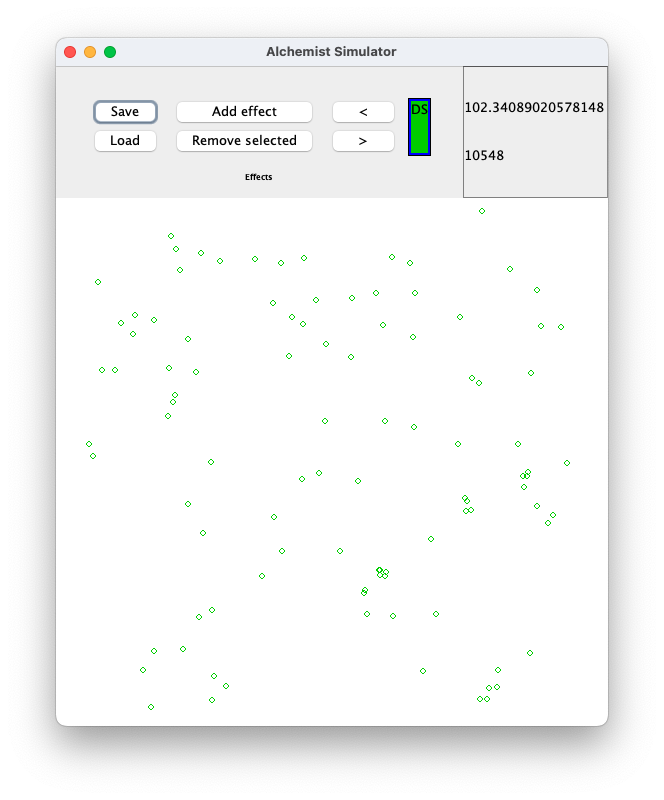
\includegraphics[width=0.32\textwidth]{figures/cento100.png}} 
    \subfigure[]{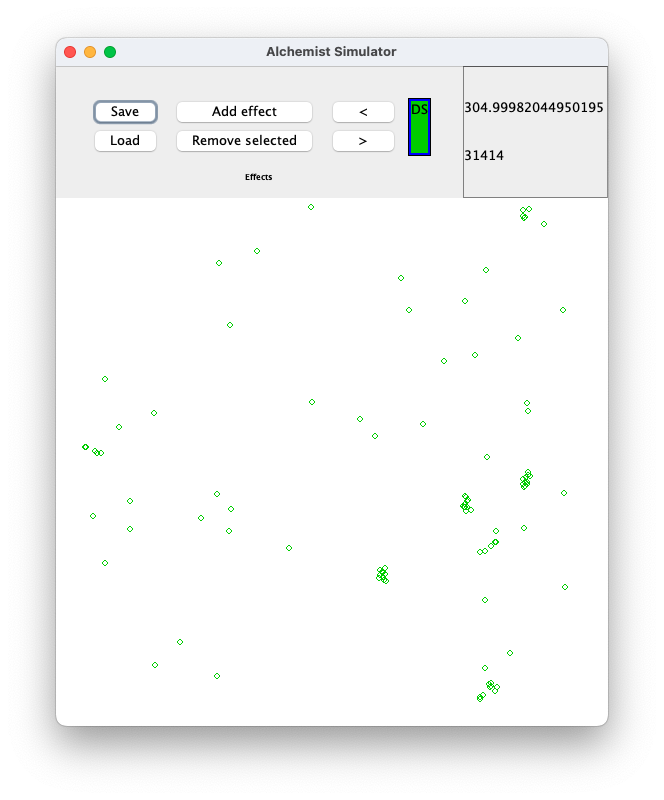
\includegraphics[width=0.32\textwidth]{figures/centoF.png}}
    \caption{(a) Inizio (b) Dopo 100 secondi (c) Dopo 300 secondi}\label{fig:sim3}
\end{figure}
\begin{figure}[ht]
    \centering
    \subfigure[]{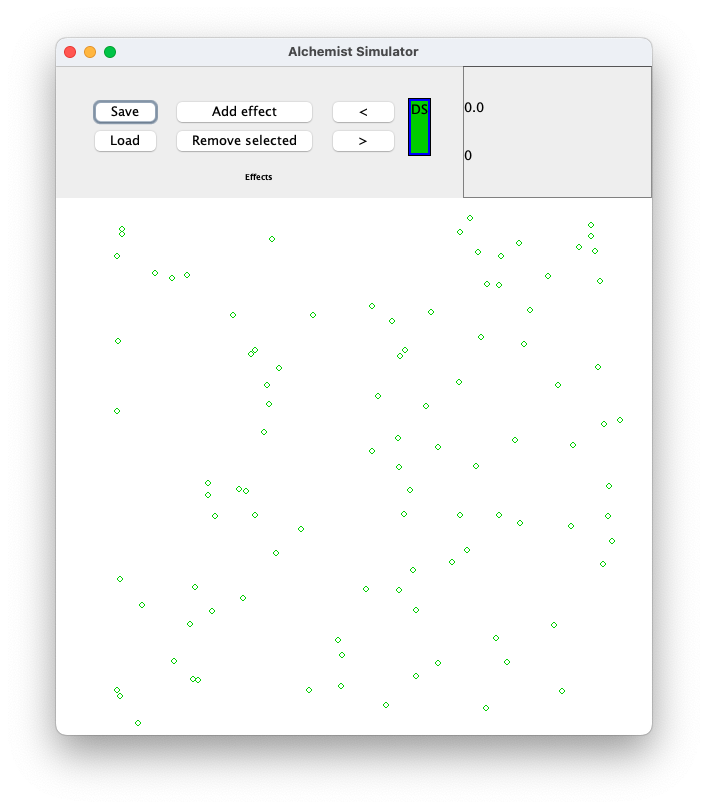
\includegraphics[width=0.32\textwidth]{figures/centoNo0.png}} 
    \subfigure[]{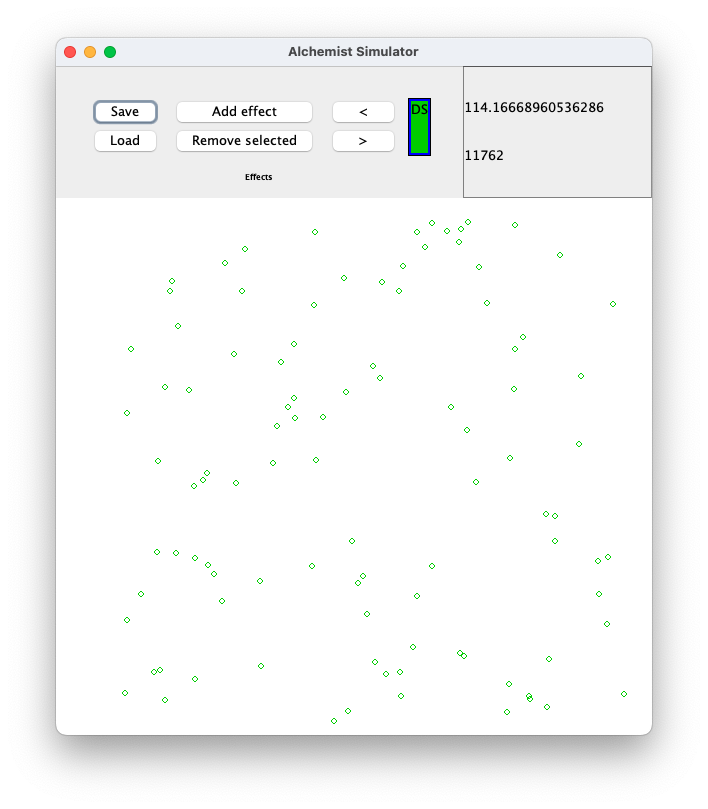
\includegraphics[width=0.32\textwidth]{figures/centoNo100.png}} 
    \subfigure[]{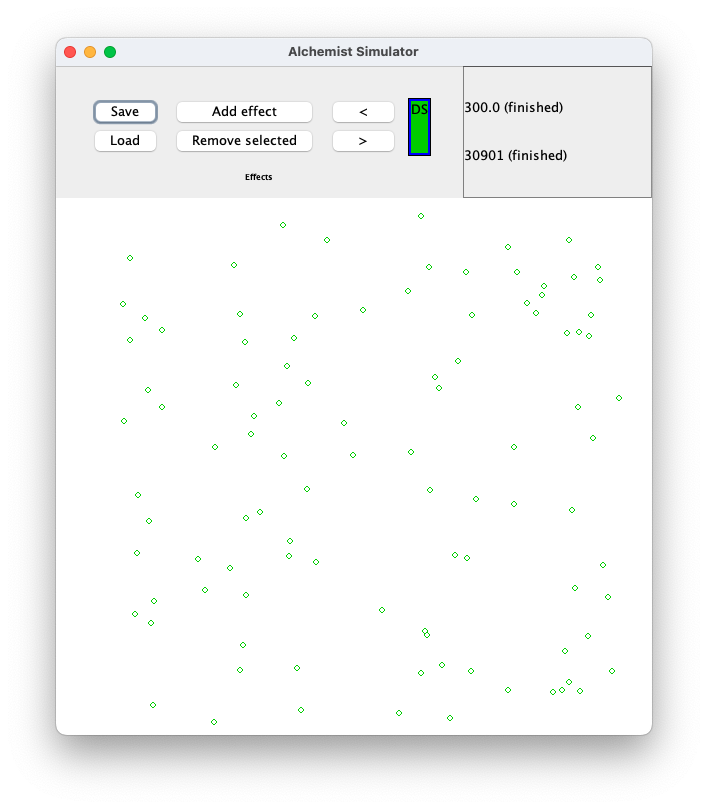
\includegraphics[width=0.32\textwidth]{figures/centoNoF.png}}
    \caption{(a) Inizio (b) Dopo 100 secondi (c) Dopo 300 secondi}\label{fig:sim4}
\end{figure}
\begin{figure}[ht]
    \centering
    \subfigure[]{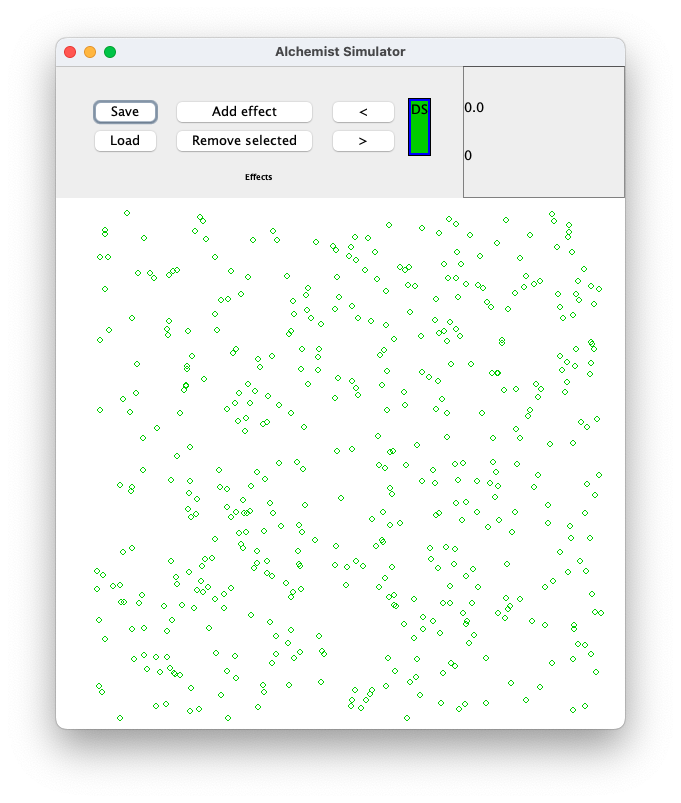
\includegraphics[width=0.32\textwidth]{figures/small0.png}} 
    \subfigure[]{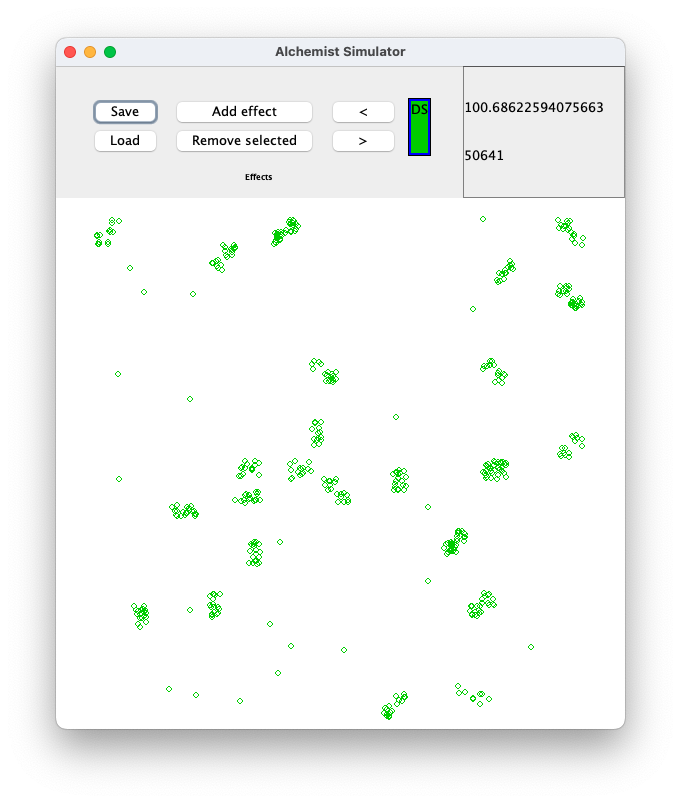
\includegraphics[width=0.32\textwidth]{figures/small100.png}} 
    \subfigure[]{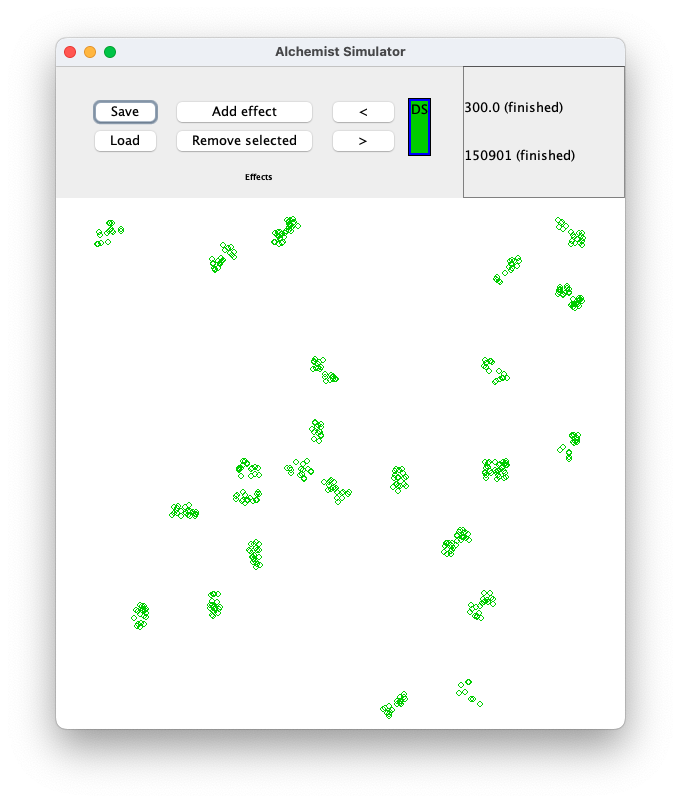
\includegraphics[width=0.32\textwidth]{figures/smallF.png}}
    \caption{(a) Inizio (b) Dopo 100 secondi (c) Dopo 300 secondi}\label{fig:sim5}
\end{figure}
\chapter{Conclusioni e lavori futuri}
\section{Conclusioni}
In questa tesi è stato presentato un modello di simulazione di comportamenti emergenti in Alchemist,
prendendo come riferimento il comportamento di aggregazione di organismi \textit{slime-mold}.
Lo svolgimento del progetto ha portato con successo lo sviluppo di sorgenti software che permettono di simulare
questo comportamento in Alchemist.
\section{Lavori futuri}
Un possibile sviluppo futuro di questo lavoro di tesi potrebbe consistere nel modificare il modello per permettere all'utente di definire l'angolo di 
scoperta del feromone. Attualmente ogni nodo ``sniffa'' il feromone a 360 gradi, ma sarebbe interessante
poter definire un angolo di visuale, in modo da poter simulare comportamenti più realistici.

\chapter{Ringraziamenti}
Innanzitutto i miei ringraziamenti vanno al mio relatore, Prof.\ Mirko Viroli, e al mio correlatore,
Dott. Gianluca Aguzzi. Grazie per avermi concesso questa opportunità.
In particolare ringrazio il Dott.\ Aguzzi per la sua infinita disponibilità e per avermi supportato durante questo percorso.
Ringrazio la mia famiglia per avermi sempre sostenuto e per avermi permesso di arrivare fin qui.

Un grazie va anche alla compagnia di Rimini per tutte le belle serate che abbiamo passato insieme.
Ringrazio anche tutti gli amici che ho conosciuto durante questo percorso e quelli che conoscevo già prima
di iniziarlo. 
Infine un grazie particolare ad Angela per avermi sempre supportato e per essere stata al mio fianco.
%----------------------------------------------------------------------------------------
% BIBLIOGRAPHY
%----------------------------------------------------------------------------------------

\backmatter\nocite{*} % comment this to only show the referenced entries from the .bib file

\bibliographystyle{alpha}
\bibliography{bibliography}

\end{document}